% !TeX document-id = {05a68193-ed62-4aec-af1e-41fca22d30e3}
% !TeX TXS-program:compile = txs:///lualatex/[-shell-escape]
% !BIB TS-program = biber
% !TeX spellcheck = nl_NL-Dutch
% TeX program = luatex
% Compilation notes:
%	- LuaLaTeX is necessary right now to support the chapter style. If not for that, pdflatex would work.
%	- To compile the index, use Tools > Index in TeXstudio after compiling once, then compile again. Don't wanna change the automatic pipeline.
\documentclass[a4paper, 11pt]{book}

%%%%%%%%%%%%%%%
%%% IMPORTS %%%
%%%%%%%%%%%%%%%
\usepackage[inner=1.5in, outer=1in, top=1in, bottom=1in]{geometry}  % Margins
%\usepackage[margin=1in]{geometry}  % Margins
\usepackage{parskip}    % No LaTeX indents, and empty lines between paragraphs in .tex files translate to stretchy-but-not-too-big blank lines in the PDF output.

% Math
\usepackage{mathtools}  % Math things
\usepackage{amssymb}    % More math things
%\usepackage{unicode-math}  % Extends amssymb with \mathbb{1} and other stuff. Note: changes all other math and clashes with rsfso.
\usepackage{dsfont}     % Double-stroked letters like \mathds{1}
\usepackage{mathdots}   % Dotty math things
\usepackage{bm}         % Bold math
\usepackage[scr]{rsfso} % Sexy \mathscr capitals
\usepackage{siunitx}    % Units
\usepackage{commath}    % Derivative and integral d's, and also norms.
\usepackage{interval}   % Standardised intervals (European convention, separators ...)
\usepackage{xspace}     % An optional space \xspace behind 0-argument commands.
\usepackage{amsthm}     % Basic theorems

% Figures
\usepackage{graphicx}   % Figures
\usepackage{float}      % [H] placement
\usepackage{mdframed}   % Theorem (example, exercise ...) environments with frames, leftrules ...
\usepackage{changepage} % For \begin{adjustwidth}{-...}{-...} to eat into margins.
\usepackage{pdflscape}  % Landscape pages, but unlike lscape, these actually rotate in the PDF too.
\usepackage[margin=10pt,font=small,labelfont=bf,labelsep=endash]{caption}    % Needed for two purposes: 1. to put tables and figures inside mdenvs, and 2. for syling captions.
\usepackage{subcaption} % Subfigures
\usepackage[svgnames,table]{xcolor}     % Colours. svgnames is for some title themes.
\usepackage{tikz}
\usetikzlibrary{calc}
\usetikzlibrary{matrix}       % For Viterbi trellis
\usetikzlibrary{positioning}
\usepackage[edges]{forest}  % Easy syntax for trees. The "edges" option allows rectangular branches as a style option.
\usepackage[noend]{algpseudocode}  % Algorithm syntax
\usepackage[algochapter]{algorithm}             % Algorithm float
\usepackage{neuralnetwork}  % Viterbi in appendix
\usepackage{menukeys}   % Used in a footnote to explain WebCelex menu steps.
\usepackage{minted}

% Tables
\usepackage{multirow}  % Split table cells
\usepackage{makecell}  % Breakable cells
\usepackage{longtable} % Big ol' table, at least 7 inches no cap. Load before arydshln if you don't want to cry.
\usepackage{hhline}    % Double table lines
\usepackage{arydshln}  % Dashed table lines

% Typography
%\usepackage[utf8]{inputenc}
\usepackage{fontspec}  % Allows Greek text inclusion (example: The Greek word {\fontspec{Linux Libertine O}ἐπιστήμη} means ``science''.)
\usepackage[dutch]{babel}
\usepackage[style=english]{csquotes}\MakeOuterQuote{"}  % Easy quotes

% Links
\usepackage{imakeidx}    % To get an index. Must be loaded before hyperref: https://tex.stackexchange.com/a/22014/203081
\usepackage{hyperref}
\usepackage[backend=biber, 
	defernumbers=true,  % "defernumbers" means that if you print the bibliography in multiple pieces, their numbering (if you use IEEE style) will be sorted according to how they are printed, and NOT according to how they would be printed if there was one big bibliography.
	style=authoryear, citestyle=authoryear,
	maxbibnames=99, 
	maxcitenames=2,     % Cite either 1 author, 2 authors, or 1 author + et al.
	uniquelist=false,    % Solves issue where for the same author but a different year, the author names are still disambiguated. https://tex.stackexchange.com/q/676517/203081. Also solves issues with same author same year, see the examples in section 4.11.4.1 and 4.11.4.2 of the manual at https://mirror.lyrahosting.com/CTAN/macros/latex/contrib/biblatex/doc/biblatex.pdf. Note: "uniquelist" only takes effect when biber compiles again.
	uniquename=false,  % To prevent Chinese names from getting a first name like "S Wang" and "Yingting Wu" because there are so many authors with the same last name. https://tex.stackexchange.com/q/321460/203081
	dashed=false  % If true, the bibliography puts a ---- in place of the authors if they are the same as in the previous entry.
]{biblatex}

% Attachments
\usepackage{pdfpages}   % For the cover
\usepackage[titletoc]{appendix}          % "Appendix" prefix in ToC.
%\usepackage[printwatermark]{xwatermark}  % "DRAFT" watermark. But nevermind, this package is evil.  https://tex.stackexchange.com/a/581962/203081
%\usepackage{todonotes}  % This package is evil and will never work, so I defined my own version in Commands.
\makeindex[options={-s pre/IndexStyle.ist}]  % Like \makeglossary. Style of the index defined at https://tex.stackexchange.com/q/530376/203081. NOTE: in TeXstudio, to recompile the index, use Tools > Index!
\usepackage[totoc]{idxlayout}   % Index in the ToC. https://tex.stackexchange.com/a/57437/203081

%%%%%%%%%%%%%%%%%%%%%%
%%% PREAMBLE PARTS %%%
%%%%%%%%%%%%%%%%%%%%%%
%%%%%%%%%%%%%%%%%%%%%%%
%%% CUSTOM SETTINGS %%%
%%%%%%%%%%%%%%%%%%%%%%%
% Language-specific title strings.
% -- New names
\newcommand{\algorithmname}{Algorithm}
\newcommand{\abstractname}{Abstract}
\newcommand{\cruxname}{Crux}
\newcommand{\illustrationsname}{Lists of illustrations}

% -- Language-specific changes
\addto\captionsdutch{
	\renewcommand{\abstractname}{Abstract}
	\renewcommand{\appendixname}{Appendix}      % Shown at start of appendix chapter
	\renewcommand{\bibname}{Bibliografie}
	\renewcommand{\chaptername}{Hoofdstuk}      % Shown at start of main chapter
	\renewcommand{\contentsname}{Inhoudstafel}  % Shown above ToC
	\renewcommand{\figurename}{Figuur}          % Shown in caption, not in inline reference
	\renewcommand{\indexname}{Index}
	\renewcommand{\listfigurename}{Figurenlijst}
	\renewcommand{\listtablename}{Tabellenlijst}
	\renewcommand{\listalgorithmname}{Algoritmenlijst}
	\renewcommand{\partname}{Deel}              % Shown on inserted part sheet
	\renewcommand{\refname}{Referenties}
	\renewcommand{\tablename}{Tabel}            % Shown in caption, not in inline reference
	\renewcommand{\algorithmname}{Algoritme}  % Idem.
	\renewcommand{\cruxname}{Samengevat}
	\renewcommand{\illustrationsname}{Lijsten van illustraties}
}

% Inline referencing:
% - For sections, figures, and tables, use \autoref{}.
% - For parts, use \fullref{}.

% -- First define spacers that ensure an exact amount of space is put after the autoref names (for which you have to gobble the space that would exist after).
\makeatletter  % This is here to activate @-commands.
\def\fixedsectionspace{\kern1pt\@gobble}
\def\fixedeqspace{\kern1.25pt\@gobble}
\makeatother

% -- New names
\def\algorithmlineautorefname{line}%

% -- Language-specific changes
\addto\extrasenglish{%  % These all appear inline.
	\def\sectionautorefname{\S{}\fixedsectionspace}%
	\def\subsectionautorefname{\S{}\fixedsectionspace}%
	\def\subsubsectionautorefname{\S{}\fixedsectionspace}%
	\def\paragraphautorefname{\S{}\fixedsectionspace}%
	\def\subparagraphautorefname{\S{}\fixedsectionspace}%
}

\addto\extrasdutch{%  % These all appear inline
	\def\sectionautorefname{\S{}\fixedsectionspace}%
	\def\subsectionautorefname{\S{}\fixedsectionspace}%
	\def\subsubsectionautorefname{\S{}\fixedsectionspace}%
	\def\paragraphautorefname{\S{}\fixedsectionspace}%
	\def\subparagraphautorefname{\S{}\fixedsectionspace}%
	%
	\def\partautorefname{Deel}%
	\def\chapterautorefname{Hoofdstuk}%
	\def\appendixautorefname{Appendix}%
	\def\figureautorefname{Figuur}%
	\def\tableautorefname{Tabel}%
	\def\pageautorefname{pagina}%
	%
	\def\equationautorefname{Vgl.}%   % For safety using \autoref on accident. Use \eqref.
	\def\thmautorefname{Stelling}%
	\def\defiautorefname{Definitie}%
	\def\questionautorefname{Onderzoeksvraag}%
	\def\algorithmlineautorefname{lijn}%
	\def\algorithmautorefname{Algoritme}%
    \def\pageautorefname{pagina}%
}

%%%%%%%%%%%%%%%%%%%%%%%%%%%%%%%%%%%%%%%%%%%%%%%%%%%%%%%%%%%%%%%%

% No double space after period. It stretches too much IMHO. https://tex.stackexchange.com/questions/4705/double-space-between-sentences
\frenchspacing

% Hyperref
\definecolor{skyblue}{HTML}{009BCF}
\definecolor{deepgreen}{HTML}{399A0C}
\definecolor{cerulean}{HTML}{00A2E3}
\hypersetup{
    colorlinks=true,
    urlcolor=cerulean,
    citecolor=deepgreen,
    linkcolor=Purple
}

% Footnotes keep counting over chapters
\counterwithout*{footnote}{chapter}

% Section numbering for subsub
\setcounter{secnumdepth}{3}

% Remove the unwanted space \left( and \right) generate by default (e.g., \cos\left(a\right) renders as cos (a) instead of cos(a); this is very apparent when using E[] and Var[] in probtheory) (https://tex.stackexchange.com/q/2607/203081)
\let\originalleft\left
\let\originalright\right
\renewcommand{\left}{\mathopen{}\mathclose\bgroup\originalleft}
\renewcommand{\right}{\aftergroup\egroup\originalright}

% Interval configuration
\intervalconfig{
	separator symbol = {;}	
}

% mdframed spacing
\mdfsetup{skipabove=6pt,skipbelow=5pt}

% minted gray line numbers
\renewcommand{\theFancyVerbLine}{\textcolor[rgb]{0.85,0.85,0.85}{\tiny\arabic{FancyVerbLine}}}

% Footnotes that escape from frame environments: \footnoteof{}. For having floats inside these environments, use \captionof{thefloattype}{thecaption}\label{thelabel}.
\usepackage{tablefootnote} 
\makeatletter
\AfterEndEnvironment{mdframed}{%
	\tfn@tablefootnoteprintout% 
	\gdef\tfn@fnt{0}% 
}
\makeatother 
\newcommand{\footnoteof}[1]{\tablefootnote{#1}}

% Bold table heads
\renewcommand\theadfont{\bfseries}

% Configure \hdashline to be dotted instead of dashed (https://tex.stackexchange.com/a/169103/203081)
\setlength{\dashlinedash}{0.25pt}
\setlength{\dashlinegap}{0.75pt}
%\setlength{\arrayrulewidth}{1pt}

% Make pages red if they exceed the thesis page limit (https://tex.stackexchange.com/a/675875/203081). Note: \AddToHook needs at least LaTeX 2020 installed. Some newer LaTeX versions crash for some packages, so this might also help: https://tex.stackexchange.com/a/581962/203081.
%\usepackage{afterpage}
%\usepackage{etoolbox}
%\AddToHook{shipout/before}{
%    \ifnum\ReadonlyShipoutCounter=70
%        \pagecolor{red}
%    \else
%        \relax
%    \fi
%}

% Tokenisation tree style
\newcommand\forestskip{1 mm}
\forestset{
    % Configure tree so it can be stacked with other trees: https://tex.stackexchange.com/a/687344/203081
    bpetree/.style = {
        delay={where content={}{shape=coordinate}{}},
        where n children=0{
        	tier=word, 
        	baseline,
        	font=\scshape
        }{},
        for tree={
            text height = 2ex,
            text depth  = 0.5ex,
            inner ysep = 0pt,
            inner xsep = 1pt,
            s sep = \forestskip + 1mm
        },
        % Drop nodes as low as possible: https://tex.stackexchange.com/a/686577/203081
        for tree children-first={
          if n children=0{
            tier=0,
          }{
            tier/.max={1+tier}{children},
          },
        },
        forked edges
    }
}
%%%%%%%%%%%%%%%%%%%%%%%
%%% CUSTOM COMMANDS %%%
%%%%%%%%%%%%%%%%%%%%%%%
\usepackage{suffix}

% \fullref command outputting a link with the autoref link AND the full name of whatever is linked; practically, this is most useful for referencing parts (e.g. `Part III: Statistics')
\newcommand*{\fullref}[1]{\hyperref[{#1}]{\autoref*{#1}: \nameref*{#1}}}

% \emph*, which applies \emph and adds its content to the index. https://tex.stackexchange.com/a/50773/203081
\WithSuffix\newcommand\emph*[1]{\emph{#1}\index{#1}}

% The current and next year
\def\thisyear{\the\numexpr\year+0\relax}
\def\nextyear{\the\numexpr\year+1\relax}

% Scaling in math mode (use in math mode, and specifying a scale factor i.o. a length)
\newcommand\scalemath[2]{\scalebox{#1}{\mbox{\ensuremath{\displaystyle #2}}}}

% Small separation line
\newcommand*\segsep{% Use most times
	\vspace{-0.6em}\\\rule{1cm}{0.4pt}\\
}

% Font size between \tiny and \scriptsize (https://tex.stackexchange.com/a/432684/203081)
\makeatletter
\newcommand\notsotiny{\@setfontsize\notsotiny\@vipt\@viipt}
\makeatother

% Math
\newcommand\Log[1]{\mathop{{}^{#1}\!\log}}  % Benelux logarithm
\renewcommand{\emptyset}{\varnothing}  % The better emptyset
\newcommand{\D}{\mathcal{D}}
\newcommand{\T}{\mathcal{T}}
\newcommand{\N}{\mathbb{N}}
\newcommand{\R}{\mathbb{R}}
\newcommand{\E}{\mathbb{E}}
\newcommand{\ft}{\mathfrak{t}}  % fraktur t
\newcommand{\elltwo}{\mathbb{L}^{\!2}}
\newcommand{\matr}[1]{\bm{#1}}
\newcommand{\tmatr}[1]{\bm{#1}^\intercal}
\newcommand{\listindex}[1]{\co{[}#1\co{]}}
\DeclareMathOperator{\softmax}{softmax}
\DeclareMathOperator{\Li}{\mathcal{L}}
\DeclareMathOperator{\uni}{\cup}
\newcommand{\ind}[1]{{\mathds{1}}\{#1\}}  % Curly braces because square brackets without any prefix already mean "convert bool to int", so a prefix would become pleaonastic. See https://en.wikipedia.org/wiki/Iverson_bracket
\renewcommand{\Re}{\text{Re}}  % Ain't nobody got time for RealPart(). I use it for recall.

% Easy superscript for centuries, e.g. 20\up{th}
\let\up\textsuperscript
\let\down\textsubscript

\usepackage{relsize}
\renewcommand{\_}{\textscale{.5}{\textunderscore}}  % Shorter underscore https://tex.stackexchange.com/a/128817/203081. DO NOT USE THIS IN MATH MODE, IT WILL CRASH THE COMPILER AND TEXSTUDIO.
\newcommand{\specialtoken}[1]{\langle \texttt{#1}\rangle}
\newcommand{\unk}{\specialtoken{UNK}}
\newcommand{\eos}{\specialtoken{EOS}}
\newcommand{\sow}{\textsc{sow}\xspace}
\newcommand{\eow}{\textsc{eow}\xspace}
\newcommand{\ellipsis}{\textsc{[...]}\xspace}

% Text styles
\newcommand{\ex}[1]{\textsl{#1}}   % Example
\newcommand{\co}[1]{\texttt{#1}}   % Code
\newcommand{\lxm}[1]{\textsc{#1}}  % Lexeme
\newcommand{\tk}[1]{\textsf{#1}}   % Tokeniser
\newcommand{\textgreek}[1]{{\fontspec{Linux Libertine O}#1}}
\newcommand{\textrussian}[1]{{\fontspec{Linux Libertine O}#1}}
\newcommand{\textchinese}[1]{{\fontspec{Linux Libertine O}#1}}

% Hebrew support (any/all of these statements are necessary; took me a long time to throw this together)
\babelfont[hebrew]{rm}{SILEOT.ttf}  % You need to install this. Overleaf has it automatically. https://software.sil.org/ezra/
\babelprovide[onchar=fonts ids]{hebrew}  % This should allow writing Hebrew Unicode without wrapping it in \texthebrew 
\DeclareLanguageMapping{hebrew}{english}  % This means BibLaTeX doesn't complain about "language not supported".
\newcommand{\texthebrew}[1]{\foreignlanguage{hebrew}{#1}}

% Abbreviations
\newcommand{\bert}{\textsc{bert}\xspace}
\newcommand{\roberta}{Ro\textsc{BERT}a\xspace}
\newcommand{\robbert}{Rob\textsc{BERT}\xspace}
\newcommand{\berttiny}{\textsc{bert}\textsubscript{\textsc{tiny}}\xspace}
\newcommand{\gptFour}{\textsc{gpt-4}\xspace}
\newcommand{\gptThree}{\textsc{gpt-3}\xspace}
\newcommand{\gptTwo}{\textsc{gpt-2}\xspace}
\newcommand{\gpt}{\textsc{gpt}\xspace}
\newcommand{\bleu}{\textsc{bleu}\xspace}
\newcommand{\bpe}{\textsc{bpe}\xspace}
\newcommand{\wpm}{\textsc{wpm}\xspace}
\newcommand{\bpeNL}{\textsc{bpe}\down{nl}\xspace}
\newcommand{\repo}{\textsc{bauwemt}\xspace}

% Wikipedia superscripts
\newcommand{\eng}{Eng.:\,}  % To be used explicitly without braces (\eng, not \eng{})
\newcommand{\ned}{Ned.:\,}
\newcommand{\cn}{\textsuperscript{\color{blue}[citation needed]}}

% Support Unicode characters ⸤ and ⸥ (https://tex.stackexchange.com/a/679336/203081)
\usepackage{newunicodechar}
\newfontface{\lowbrackets}{Noto Sans}
\NewDocumentCommand{\blhb}{}{{\lowbrackets\symbol{"2E24}}}
\NewDocumentCommand{\brhb}{}{{\lowbrackets\symbol{"2E25}}}
\newunicodechar{⸤}{\blhb}
\newunicodechar{⸥}{\brhb}

% Combine list of figures and tables. Generalised version of https://tex.stackexchange.com/a/14545/203081
\makeatletter
\providecommand\phantomsection{}% for hyperref
\newcommand{\listofillustrations}{%
	\chapter{\illustrationsname}%
	\phantomsection
	%\addcontentsline{toc}{chapter}{Lijst van illustraties}%
	\section*{\listfigurename}%
	\phantomsection
	\addcontentsline{toc}{section}{\listfigurename}%
	\@starttoc{lof}%
	\bigskip
	\section*{\listtablename}%
	\phantomsection
	\addcontentsline{toc}{section}{\listtablename}%
	\@starttoc{lot}%
	\bigskip
	%\section*{\listalgorithmname}%
	%\phantomsection
	\addcontentsline{toc}{section}{\listalgorithmname}%
	% So, for some reason, \@starttoc{loa} doesn't want to work (it outputs garbled titles). Luckily I found this fix https://tex.stackexchange.com/a/198860/203081 as an alternative. It lets \listofalgorithms do its thing as usual, except we ninja-edit \chapter* to be \section*.
	\begingroup
	\let\chapter\section% Temporary
	\listofalgorithms
	\endgroup
	%\@starttoc{loa}%
}
\makeatother

% Todonotes that doesn't kill you when you include it. TODO: Could be better, e.g. anti-overlap.
\let\marginnote\someundefinedcommand
\usepackage{marginnote}
%\reversemarginpar
\newcommand{\marginboxTB}[2]{\marginnote{%
	\begin{tikzpicture}%
		\node[draw,fill=#1,align=left,rounded corners,text width=0.5\marginparwidth] () {#2};%Need to align=... to be breakable. https://tex.stackexchange.com/a/31100/203081
	\end{tikzpicture}}[-1.75em]}% Move up by one line.

\newcommand{\todo}[1]{\marginboxTB{red!15}{#1}}

% --- Gradient-coloured table cells: surround cell content by \tgrad. Based on a mix of answers at https://tex.stackexchange.com/q/174998/203081.
\usepackage{pgf}
\usepackage{etoolbox}

% Definitions
\newcommand*{\MinNumber}{0.0}%
\newcommand*{\MidNumber}{0.5} %
\newcommand*{\MaxNumber}{1.0}%

\definecolor{high}{HTML}{03AC13}
\definecolor{mid}{HTML}{F7E379}
\definecolor{low}{HTML}{ec462e}
\newcommand*{\cellopacity}{80}

% Cell command
\newcommand{\tgrad}[1]{%
    \ifdim #1 pt > \MidNumber pt%
        \pgfmathparse{max(min(100.0*(#1 - \MidNumber)/(\MaxNumber-\MidNumber),100.0),0.00)}%
        \xdef\PercentColor{\pgfmathresult}%
        \cellcolor{high!\PercentColor!mid!\cellopacity}#1%
    \else
        \pgfmathparse{max(min(100.0*(\MidNumber - #1)/(\MidNumber-\MinNumber),100.0),0.00)}%
        \xdef\PercentColor{\pgfmathresult}%
        \cellcolor{low!\PercentColor!mid!\cellopacity}#1%
    \fi
}

% Optional: add a new tabular column type, "R", that applies tgrad to all cells automatically. Only works for fully numeric columns though; no column headers allowed.
%\usepackage{collcell}
%\newcolumntype{R}{>{\collectcell\tgrad}c<{\endcollectcell}}

%%%%%%%%%%%%%%%%%%%%%%%%%%%
%%% CUSTOM ENVIRONMENTS %%%
%%%%%%%%%%%%%%%%%%%%%%%%%%%

% Chapter abstract
\newenvironment{abstract}{
	\begin{quote}
		\small \textbf{\abstractname~--}
}{
	\end{quote}
}

% Crux
\newenvironment{crux}{
	\begin{quote}
		\small \textbf{\cruxname~--}
}{
	\end{quote}
}

% Generic style for boxes.
\mdfdefinestyle{basic}{%
	backgroundcolor=black!5,
    linewidth=1pt,
    frametitlebelowskip=-0.25\topskip,
   	skipbelow=-0.12em
}


% Box with INLINE title. Taken from MCS book.
\newtheoremstyle{question}{-\topsep}{}{\slshape}{}{\bfseries}{}{.5em}{}
\theoremstyle{question}  % All theorem declarations after this will have this style.
\newmdtheoremenv[  % Not mdtheorem! https://tex.stackexchange.com/q/655399/203081
	default,
	skipabove=0.5em,
	linewidth=1pt
]{question}{\questionname}%[part]

% Lined quote. Taken from K&S book.
\mdfdefinestyle{leftrule}{%
	topline=false,
	bottomline=false,
	rightline=false,
	linewidth=1.25pt,
	skipbelow=-0.12em
}
\renewmdenv[style=leftrule, font=\small]{blockquote}

% Parent style of all styles. \mdfsetup doesn't seem to be able to regulate spacing if the "default" option is used, so my solution is to let all other styles inherit the same spacing settings.
% (not sure why I commented them out, but they're here when you need them!)
%\mdfdefinestyle{spacing}{
%	skipabove=0.5em,
%	frametitlebelowskip=-0.25\topskip
%}
%\mdfdefinestyle{dashed}{%
%	style=spacing,
%	linecolor=white, 
%	tikzsetting={draw=black, dashed, line width=1pt, dash pattern=on 5pt off 5pt}
%}
%\mdfdefinestyle{dotted}{%
%	style=spacing,
%	linecolor=white, 
%	tikzsetting={draw=black, dotted, line width=1pt}
%}
%\newcommand{\dashedboxReducedwidthUnnumbered}[2]{
%	\begin{mdframed}[default, style=dashed, userdefinedwidth=0.75\linewidth, align=center]
%		\textbf{#1}\\
%		#2
%	\end{mdframed}
%}

% Horizontal+vertical center
\newenvironment{fullcenter}{
	\mbox{}\vfill\begin{center}
}{
	\end{center}\vfill\mbox{}
}

% subequations*: amsmath's subequations, but continuing the equations' number since the last subequations/subequations* so you can have something like equation 1a, 1b, 2, and then later 1c. (https://tex.stackexchange.com/a/101004/203081)
\makeatletter
\newcounter{qrr@oldeq}
\newcounter{qrr@oldsubeq}
\newcounter{qrr@realeq}
\renewenvironment{subequations}{%
	\refstepcounter{equation}%
	\protected@edef\theparentequation{\theequation}%
	\setcounter{parentequation}{\value{equation}}%
	\setcounter{equation}{0}%
	\def\theequation{\theparentequation\alph{equation}}%
	\ignorespaces
}{%
	\setcounter{qrr@oldeq}{\value{parentequation}}%
	\setcounter{qrr@oldsubeq}{\value{equation}}%
	\setcounter{equation}{\value{parentequation}}%
	\ignorespacesafterend
}
\newenvironment{subequations*}{%
	\setcounter{qrr@realeq}{\value{equation}}%
	\let\theparentequation\theequation%
	\patchcmd{\theparentequation}{equation}{parentequation}{}{}%
	\setcounter{parentequation}{\numexpr\value{qrr@oldeq}-1}%
	\setcounter{equation}{\value{qrr@oldsubeq}}%
	\def\theequation{\theparentequation\alph{equation}}%
	\refstepcounter{parentequation}%
	\ignorespaces
}{%
	\setcounter{qrr@oldeq}{\value{parentequation}}%
	\setcounter{qrr@oldsubeq}{\value{equation}}%
	\setcounter{equation}{\value{qrr@realeq}}%
	\ignorespacesafterend
}
\makeatother

% Algorithms with lines in the indents. https://tex.stackexchange.com/a/351363/203081
\usepackage{etoolbox}
\newcommand{\algruledefaultfactor}{.75}
\newcommand{\algstrut}[1][\algruledefaultfactor]{\vrule width 0pt
depth .25\baselineskip height #1\baselineskip\relax}
\newcommand*{\algrule}[1][\algorithmicindent]{\hspace*{.5em}\vrule\algstrut
\hspace*{\dimexpr#1-.5em}}

\makeatletter
\newcount\ALG@printindent@tempcnta
\def\ALG@printindent{%
    \ifnum \theALG@nested>0% is there anything to print
    \ifx\ALG@text\ALG@x@notext% is this an end group without any text?
    % do nothing
    \else
    \unskip
    % draw a rule for each indent level
    \ALG@printindent@tempcnta=1
    \loop
    \algrule[\csname ALG@ind@\the\ALG@printindent@tempcnta\endcsname]%
    \advance \ALG@printindent@tempcnta 1
    \ifnum \ALG@printindent@tempcnta<\numexpr\theALG@nested+1\relax% can't do <=, so add one to RHS and use < instead
    \repeat
    \fi
    \fi
}%

\patchcmd{\ALG@doentity}{\noindent\hskip\ALG@tlm}{\ALG@printindent}{}{\errmessage{failed to patch}}
\AtBeginEnvironment{algorithmic}{\lineskip0pt}

% Renumber with chapter (https://tex.stackexchange.com/a/124957/203081)
\makeatletter 
\renewcommand\thealgorithm{\thechapter.\arabic{algorithm}} 
\@addtoreset{algorithm}{chapter} 
\makeatother

% Add \autoref prefix to algorithm line references (name defined in Settings.tex) (https://tex.stackexchange.com/a/351229/203081)
%\makeatletter
%\patchcmd{\ALG@step}{\addtocounter{ALG@line}{1}}{\refstepcounter{ALG@line}}{}{}
%\newcommand{\ALG@lineautorefname}{\algorithmlineautorefname}
%\makeatother

% My own version (documented at https://tex.stackexchange.com/a/687624/203081), which actually works for multiple algorithms:
% - Define your own counter of which you know it isn't forced to 0 when an algorithm is started.
% - Link this counter to the algorithm counter, so that it starts over with a new algorithm (like subsections start over)
%   yet the link is stored by the counter to not produce the same ref as before.
\newcounter{algoline}[algorithm]
\renewcommand{\thealgoline}{\arabic{algoline}}

\makeatletter
\patchcmd{\ALG@step}{\addtocounter{ALG@line}{1}}{\stepcounter{ALG@line}\refstepcounter{algoline}}{}{}
\newcommand{\algolineautorefname}{\algorithmlineautorefname}
\makeatother

% Redefine name at the top of the algorithm environment (name defined in Settings.tex)
\makeatletter
\renewcommand{\ALG@name}{\algorithmname}
\makeatother


\newcommand*\Let[2]{\State #1 $\gets$ #2}
\newcommand*\Stateh{\State \algstrut[1]}  % Came with the lines-in-algorithms code.
\newcommand{\Statey}{\vspace{-0.31em}\State}  % \State tends to have a gap above it. This is another way to solve that.
%%%%%%%%%%%%%%%%%
%%% WATERMARK %%%
%%%%%%%%%%%%%%%%%
% A watermark for the first page (if you need it in the foreground, use *; if you need it on all pages, use option "allpages")
% Sadly, the xwatermark package causes the error of https://tex.stackexchange.com/q/581907/203081, so I can't use it.
%\newwatermark*[allpages,color=red!50,angle=45,scale=3,xpos=0,ypos=0]{DRAFT}
%\newwatermark[firstpage,color=red!50,angle=40,scale=4,xpos=0,ypos=5em]{DRAFT}

%\usepackage{etoolbox}
%\patchcmd{\part}{\thispagestyle{plain}}{\thispagestyle{empty}\addtocounter{page}{-1}}{}{}
%\makeatletter
%\renewcommand\@endpart{}
%\makeatother

%%%%%%%%%%%%%%%%%
%%% HEAD/FOOT %%%  ---> NOTE: The ones in the PDF are native to the book class. No fancyhdr currently!
%%%%%%%%%%%%%%%%%
%\usepackage{fancyhdr}
%\pagestyle{fancy}
%\fancyhf{}
%\renewcommand{\headrulewidth}{0pt}
%\renewcommand{\footrulewidth}{0.5pt}
%\lfoot{\textit{Kansrekenen \& statistiek} -- Handboek}
%\rfoot{\thepage}


%%%%%%%%%%%%%%%%%%%%%%%%
%%% CHAPTER HEADINGS %%%
%%%%%%%%%%%%%%%%%%%%%%%%
\usepackage[explicit]{titlesec}
\usepackage{apptools}

% Taken from https://tex.stackexchange.com/a/724738/203081
\def\firstcharacter#1{\expandafter\firstcharacterA#1{}\end}
\def\firstcharacterA#1#2\end{#1}

\titleformat{\chapter}
	[display]
	{\normalfont\bfseries}
	{\fontsize{100}{120}\selectfont\color{LightGray}\IfAppendix{}{\firstcharacter{\chaptername}}\thechapter}
	{-75pt}
	{\fontsize{28}{26}\selectfont #1}
	[]  		  % Need LuaLaTeX. Don't know why.
% --- INLINE CITATIONS ---
% Add a comma in \cite and \parencite
\renewcommand*{\nameyeardelim}{\addcomma\space}

% Make a new command to specifically only cite 1 author (counterpart of \fullcite) (https://tex.stackexchange.com/a/333958/203081)
\newcommand{\textcitefirst}[1]{%
	\AtNextCite{\defcounter{maxnames}{1}\defcounter{minnames}{1}}%
	\textcite{#1}%
}

% Make the name AND the year hyperlinked, not just the year. https://tex.stackexchange.com/a/27107/203081
\DeclareFieldFormat{citehyperref}{%
	\DeclareFieldAlias{bibhyperref}{noformat}% Avoid nested links
	\bibhyperref{#1}}

\DeclareFieldFormat{textcitehyperref}{%
	\DeclareFieldAlias{bibhyperref}{noformat}% Avoid nested links
	\bibhyperref{%
		#1%
		\ifbool{cbx:parens}
		{\bibcloseparen\global\boolfalse{cbx:parens}}
		{}}}

\savebibmacro{cite}
\savebibmacro{textcite}
\renewbibmacro*{cite}{%
	\printtext[citehyperref]{%
		\restorebibmacro{cite}%
		\usebibmacro{cite}}}

\renewbibmacro*{textcite}{%
	\ifboolexpr{
		( not test {\iffieldundef{prenote}} and
		test {\ifnumequal{\value{citecount}}{1}} )
		or
		( not test {\iffieldundef{postnote}} and
		test {\ifnumequal{\value{citecount}}{\value{citetotal}}} )
	}
	{\DeclareFieldAlias{textcitehyperref}{noformat}}
	{}%
	\printtext[textcitehyperref]{%
		\restorebibmacro{textcite}%
		\usebibmacro{textcite}}}

% Solve the issue where putting a citation in a section/chapter name incorrectly causes the citation key to become uppercased in the page header BEFORE being turned into a citation, and hence the key can't be replaced and you are left with a missing citation in the header. https://tex.stackexchange.com/a/170994/203081
\AddToNoCaseChangeList{\parencite \textcite}


% --- BIBLIGRAPHY LIST ---
% Add a little more space between bib entries.
\setlength\bibitemsep{0.5em}

% Make all authors, not just the first, be cited in reverse order.
\DeclareNameAlias{sortname}{last-first}

% Used to split the bibliography into "cited" and "not cited" automatically https://tex.stackexchange.com/a/6977/203081
\DeclareBibliographyCategory{cited}
\AtEveryCitekey{\addtocategory{cited}{\thefield{entrykey}}}

% Remove language field (usually "en." in the items) https://tex.stackexchange.com/a/401026/203081
\AtEveryBibitem{\clearlist{language}}

%%% Actually add the bibliography (relative to main.tex) %%%
\addbibresource{./res/bib/example-bibliography.bib}
%%%%%%%%%%%%%%%%%%%%%%%%%%%%%%%%%%%%%%%%%%%%%%%%%%%%%%%%%%%%

% Ensure that sources will be printed regardless of whether they were cited in the text or not.
\nocite{*}

%%%%%%%%%%%%
%%% MAIN %%%
%%%%%%%%%%%%
\begin{document}
	\frontmatter
	\pagestyle{empty}

\newcommand{\coverpath}{./text/front/cover-generator/cover.pdf}
\IfFileExists{\coverpath}{\includepdf[pages=1]{\coverpath}}{}

\begin{titlepage}
	\begin{fullcenter}
		\LARGE \textsc{\repo: a better \LaTeX{} template for \\
		engineering master's theses than kulemt}
		
		\Large drs.\ ir.\ Thomas Bauwens

		\today
	\end{fullcenter}
\end{titlepage}
\newpage
\pagestyle{plain}

\mbox{}\vfill
{\scshape
© Copyright by KU Leuven, \thisyear.

Zonder voorafgaande schriftelijke toestemming van zowel de promotor(en) als de auteur(s) is overnemen, kopiëren, gebruiken of realiseren van deze uitgave of gedeelten ervan verboden. Voor aanvragen tot of informatie i.v.m.\ het overnemen en/of gebruik en/of realisatie van gedeelten uit deze publicatie, wend u tot de KU Leuven:
\begin{verse}
	Departement Computerwetenschappen, \\
	Celestijnenlaan {\small 200A} bus {\small 2402}, B-3001 Leuven (Heverlee), België,\\
	via tel.\ +32\! 16\! 32\! 77\! 00 of via e-mail \href{mailto:info@cs.kuleuven.be}{info@cs.kuleuven.be}
\end{verse}
Voorafgaande schriftelijke toestemming van de promotor(en) is eveneens vereist voor het aanwenden van de in dit afstudeerwerk beschreven (originele) methoden, producten, schakelingen en programma’s voor industrieel of commercieel nut en voor de inzending van deze publicatie ter deelname aan wetenschappelijke prijzen of wedstrijden.
}
\newpage

\begin{center}
	\mbox{}\vfill
	\emph{Dedicated to a person I cherish, \\ and hence deserves this dedication. We won't forget him/her.}
	\vfill
\end{center}
\newpage
% https://www.clearlingo.co.nz/blog/how-to-order-the-pages-of-a-book
\newpage

	% !TeX spellcheck = nl_NL
\chapter{Foreword}

\section*{What you should know before reading}\vspace{-0.5em}
Not much, really. It helps to have experience in \LaTeX{}, but I give sufficiently many examples to show how everything works.

\section*{Dank}\vspace{-0.5em}
Don't forget to thank everyone!

\begin{itemize}
    \item Mama, papa, brothers, sisters, pets, coke suppliers, ...
    \item Dirk Vandepitte, evidently.
\end{itemize}

Hope this template helps!

\emph{-- Your Name, \today}	
	% !TeX spellcheck = nl_NL
\chapter[Abstract]{\makebox[\linewidth]{Abstract}}
\vspace{-2.5em}\makebox[\linewidth]{\resizebox{0.9\linewidth}{1pt}{$\bullet$}}\bigskip

This is where you put your abstract. Ideally, it has the following structure (derived from the writing guide by \href{https://www.principiae.be/pdfs/TM&Th-2.0-summary.pdf}{Jean-Luc Doumont}). As an example, I have suffixed each point by a summary of the paragraphs of my own thesis abstract.
\begin{itemize}
    \item \emph{Context}: What is happening in the outside world that drove you to finding a need? (E.g.: "NLP has been booming since the advent of transformers.")
    \item \emph{Need}: Why did something have to be done? ("NLP models use tokenisers to turn text into processing units as a first step. The effect of how we do this has not been studied sufficiently.")
    \item \emph{Task}: What had to be undertaken? ("BPE, the most popular tokeniser, has known issues, but nobody has gathered these or analysed them.")
    \item \emph{Object}: What, in short, did you do, as described in this document? ("In this thesis, I set up a historical framework for subword tokenisation, verify a plethora of problems with BPE, and suggest a new augmentation. The first goal is achieved by...")

    \item \emph{Findings}: What did you discover after doing it? ("The analysis shows several fundamental drawbacks of BPE, and my augmentation is superior.")
    \item \emph{Concusion}: What does this mean with regards to the need? ("Using one tokeniser over the other does fundamentally matter, and BPE is not the best one.")
    \item \emph{Perspective}: What does the future of research hold, knowing this? ("My augmentation shows that improvement is possible, which provides exciting new research opportunities.")
\end{itemize}

This was shortened by \href{https://thomaswinters.be/}{Thomas Winters} as:

\begin{itemize}
	\item \emph{Context}: Why now? What is the background?
	\item \emph{Need}: Why you? Why is this useful to the reader?
	\item \emph{Task}: Why us? What are we solving?
	\item \emph{Object}: Why this document? How are we going to solve this?

	\item \emph{Findings}: What did we find?
	\item \emph{Conclusions}: So what? What do these results imply?
	\item \emph{Perspective}: What now? What does the future look like?
\end{itemize}

It also helps to \textbf{bold} the absolutely essential keywords of the abstract (fewer than five words, let's say) to let the reader know at a glance what your thesis is about.


\makebox[\linewidth]{\resizebox{0.9\linewidth}{1pt}{$\bullet$}}\bigskip	
	%\input{text/front/Acknowledgements.tex}
	\setcounter{tocdepth}{2}
\tableofcontents

\listofillustrations
%\listoffigures
%\listoftables
\newpage
	
	\mainmatter
	\part{\textsc{\mdseries{Achtergrond}}}\label{pt:background}
	% !TeX spellcheck = en_GB
\chapter{Introduction}\label{chap:intro}
The point of \repo is to give you a bare-bones example of what a thesis could look like. It pretends to be a short thesis itself about how to use \repo and what goes where in a thesis. You can read it as straight source code, or compile it and read it as a PDF showing what your thesis could look like in the end.

\section{What do you put in an introductory chapter?}
The introductory chapter sets the tone for the rest of the thesis, both in terms of writing style and in terms of topic. You give the uninitiated reader a first look into the world you will be studying, assuming they only know as much as someone who has passed the common core of the CS master. You establish what that world is, and lead the reader to realise that this world you describe has a need for your thesis.

What prompted me to make \repo? The fact that \texttt{kulemt} really just kinda sucks. (Don't worry if you don't know \texttt{kulemt}, it will be covered in \autoref{chap:literature}.)

\section{Rest of the document}
It is customary to end your introductory chapter with a birds-eye overview of the thesis. The difference with your abstract is that here you \emph{should} refer to specific parts/chapters, whereas you \emph{should not} discuss the conclusions you draw at the end of them.
\begin{quote}
	\fullref{pt:background} contains this chapter, a literature study about alternatives available to engineering students to lay out their thesis, and the question \repo answers.
\end{quote}
\begin{quote}
	\fullref{pt:contribution} comprises installation instructions and an overview of \repo, as well as an elaborate showcase of how to achieve certain outputs with it (for example, how to lay out algorithm pseudocode). The conclusion recaps the core ideas.
\end{quote}

In \fullref{pt:apx} you can give additional information that isn't pertinent to the main body (or just doesn't fit inside the page limit):
\begin{quote}
	\fullref{apx:neuralnetworks} gives examples of drawing neural networks.
\end{quote}

	% !TeX spellcheck = nl_NL
\chapter{Literature Study}\label{chap:literature}
In \autoref{chap:intro}, I took you through the train of thoughts that led me to publishing my thesis template. It pays to know which alternatives already exist out there.

\section{kulemt}
\href{https://eng.kuleuven.be/docs/kulemt}{\emph*{kulemt}} is the original \LaTeX{} template for \underline{e}ngineering \underline{m}aster's \underline{t}heses. Its documentation is way more convoluted than it should be, the results look mid, and it didn't even do half the things I needed it to do.

\subsection{Derivatives by other faculties}
Sadly, kulemt even has \href{https://github.com/KatelijneCaerts/Latex-template-Wetenschappen}{offspring}.

\subsection{KUL on Overleaf}
KUL actually has a presence on the public Overleaf template repository, see \href{https://www.overleaf.com/latex/templates/ku-leuven-faculty-of-engineering-science-masters-thesis-template/xbjfxrbspkvs}{here} and \href{https://www.overleaf.com/latex/templates/tagged/ku-leuven}{here}. I wouldn't trust any of these though.

	% !TeX spellcheck = nl_NL
\chapter{Problem Statement}\label{chap:questions}
Having explored all the other viable \LaTeX{} thesis templates in \autoref{chap:literature}, we automatically fall into the following research question.
\begin{question}\label{q:problems}
	Can we make a better thesis template than \textsc{kulemt}?
\end{question}
The answer to \autoref{q:problems} is obviously a resounding "yes". The rest of this document is laid out as follows:
\begin{itemize}
	\item In \autoref{chap:bauwemt}, I present my own template, \repo, and how to install it.
	\item In \autoref{chap:functionality}, I provide real examples for doing all the things you likely need in a thesis.
\end{itemize}

	\part{\textsc{\mdseries{Contributie}}}\label{pt:contribution}
	% !TeX spellcheck = en_GB
\chapter{Overview of \texttt{bauwemt}}\label{chap:bauwemt}

\section{Installation}
To get started with \repo, here's what you do:
\begin{enumerate}
	\item If you don't have a local installation of \LaTeX{}, download the latest version of TeX Live from \href{https://www.tug.org/texlive/}{TUG}.
	
	\item Install the \href{https://www.texstudio.org/}{TeXstudio} editor. Don't even bother with the TeXworks editor; it has almost no features and crashes more than TeXstudio. Overleaf will not work for your thesis since it will eventually exceed the compilation time limit, and also, Overleaf requires internet access and has no version control.\footnote{Speaking of version control: if you're on Windows and don't have Git yet, now is the time to \href{https://git-scm.com/downloads}{get it}. It is not required to use \repo, but you should absolutely track the changes in your thesis.}
	
	\item Download\footnote{Do \emph{not} fork this repo for the purpose of writing your thesis. Forks are public and you will make your thesis text available to everyone who visits \repo on GitHub.} this template off of GitHub.
	
	\item Open \co{main.tex} in TeXstudio.
	
	\item Press \keys{F5} to do a first compile. This may take multiple minutes, but eventually, the resulting PDF should appear on the right.
\end{enumerate}

\section{Folder structure}
I've seen some pretty abysmal \LaTeX{} file management over the years. You wouldn't believe where some people put preamble code, body text, and images. To ensure that your thesis does not turn into such a mess, \repo isn't just a style file you import as a \co{documentclass}, but it comes as an entire folder structure instead.

You can expect to see the following hierarchy:

\begin{BVerbatim}
	tex/
	|---main.tex
	|---pre/
	|---text/
	|   |---front/
	|   |---main/
	|   `---apx/
	`---res/
	    |---fig/
	    |---tab/
	    `---bib/
\end{BVerbatim}

The top-level folder \co{tex/} makes it such that you can host other files relevant to your thesis in a sibling folder. In my case, I also have top-level folders for \co{code/}, \co{notes/}, and for \co{presentations/}.

\co{main.tex} is the file you will compile to see your thesis. It has two purposes: to import packages, and to pull in files from the rest of the thesis.

\co{pre/} is where all the files go imported in the preamble of \co{main.tex}. These files contain definitions for new \LaTeX{} commands (e.g.\ shortcuts for some symbols) and new environments, and styles for the bibliography, the index, colours used in the thesis, chapter headings and so on. If you're not \TeX{}-savvy, this is not relevant to you.

\co{text/} is where you put all the text that goes inside the thesis. It is separated into all the boilerplate in \co{front/} of your thesis (abstract, foreword, table of contents, lists, ...), your \co{main/} chapters, and possibly any appendices in \co{apx/}.

\co{res/} is where you put files that aren't text put do go inside the thesis. It is separated into \co{fig/}ures, \co{tab/}les, and \co{bib/}liography files.

\section{Writing your thesis}
Always enter the project through \co{main.tex} so that TeXstudio knows to start compiling from there, even if you are editing a different \co{.tex} file when you press \keys{F5} (compile and show this project's PDF) or \keys{F6} (compile). To open other files, you can either open them from your file system while TeXstudio is already running and has \co{main.tex} open in one tab, or you can scroll down in \co{main.tex} to where \verb|\begin{document}| is defined and \keys{Ctrl+Lclick} the paths loaded with \verb|\input{}|.

When you are writing, it should become a habit to press \keys{Ctrl+S} at the end of every sentence, \emph{except when compilation is in progress} (because then you're modifying a file while its being read, and you may get a compilation error that applies to a Frankenstein'ed version of your thesis and hence means nothing).

You should expect compilation to take quite a while. TeXstudio does not block the editor when you are compiling, except when it makes the index and bibliography. Rather than waiting for compilation to finish, you should only compile every-so-often out of habit, and keep writing the paragraph you were busy on. Once compilation is finished, you can switch from writing your paragraph to looking at the output to verify if everything works.


\section{Troubleshooting}
Compilation errors can usually be Googled to resolve them. Always look for a link to \href{https://tex.stackexchange.com/}{tex.stackexchange.com} in the search results, because this is by far the best place to find high-quality information about \LaTeX{} features and bugs.

If you find that one of your issues is caused by \repo specifically, please \href{https://github.com/bauwenst/bauwemt/issues}{open a GitHub issue}.

	% !TeX spellcheck = nl_NL
\chapter{Functionality}\label{chap:functionality}
\begin{abstract}
If you like having a short abstract that summarises your chapters, you can add one with the \verb|abstract| environment.
%Did you ever hear the tragedy of Darth Plagueis The Wise? I thought not. It’s not a story the Jedi would tell you. It’s a Sith legend. Darth Plagueis was a Dark Lord of the Sith, so powerful and so wise he could use the Force to influence the midichlorians to create life… He had such a knowledge of the dark side that he could even keep the ones he cared about from dying. The dark side of the Force is a pathway to many abilities some consider to be unnatural. He became so powerful… the only thing he was afraid of was losing his power, which eventually, of course, he did. Unfortunately, he taught his apprentice everything he knew, then his apprentice killed him in his sleep. Ironic. He could save others from death, but not himself.
\end{abstract}

We just installed \repo in \autoref{chap:bauwemt}. Below, I showcase \emph{what} you can do with it. Because the source code for this documentation \emph{is} \repo, it shows you exactly \emph{how} to do everything that is showcased.


\section{Text style}
Paragraphs are separated by half a line of whitespace in \repo, and have no indents. In the source, you simply leave an empty line between paragraphs. No commands needed.

As usual in \LaTeX{}, it is recommended that you write what you \emph{mean}, not what to \emph{show}: don't ask "make this bold" but ask "emphasise this" and then later on decide that everything that is emphasised should be bolded (or slanted, or underlined, or made blue, etc...). In my thesis, I had commands for \emph{emphasis}, \co{code}, and \ex{examples}.

In some rare cases, you may want to hard-code the style. You can do that with:
\begin{center}
\begin{tabular}{l|l}
\bfseries Command form & \bfseries Series form \\ \hline
\verb|\textbf{...}|       & \verb|{\bfseries ...}| \\
\verb|\textit{...}|       & \verb|{\itshape ...}| \\  
\verb|\textsl{...}|       & \verb|{\slshape ...}| \\
\verb|\textsf{...}|       & \verb|{\sffamily ...}| \\
\verb|\textsc{...}|       & \verb|{\scshape ...}| \\
\verb|\textcolor{c}{...}| & \verb|{\color{c} ...}| \\ 
\verb|\underline{...}| & /
\end{tabular}
\end{center}

\section{Quotes}
\subsection{Inline quotes}
Normally, to balance quotes, you need \verb|``| and \verb|''|. This is annoying to type, and goes against the entire point of using \LaTeX{}, which again is to write what you \emph{mean}, not what to \emph{show}. Hence, \repo allows using \verb|"|, plain and simple.

\subsection{Block quotes}
To quote someone else's work correctly, it should be clear \emph{from where} and \emph{what exactly} was copied. For the latter, you can use quotation marks, but other markings work just as well. If you are Harvard's president, apparently you can water down these rules, as per \textcite{kettles_law_2023}:
\begin{blockquote}
	Harvard threatened to sue the New York Post for defamation over accusations of plagiarism against President Claudine Gay in October, calling the claims "demonstrably false." Then, the University’s own review found several instances of "duplicative language" in Gay’s work. \ellipsis Still, the summary of the review said the passages at issue, "while regrettable, did not constitute research misconduct," which had to involve "intentional deception or recklessness."
\end{blockquote}


\section{Language}
\repo comes pre-loaded with support for English and Dutch. Additionally, it provides support for including Greek (\textgreek{ὕβρις}), Russian (\textrussian{Правда}), and Hebrew (\texthebrew{יהוה}) characters, with the commands \verb|\textgreek|, \verb|\textrussian| and \verb|\texthebrew|.

You can change the main language at the top of \co{main.tex}. To adapt object names in the text (the actual "Figure", "Table", "Algorithm", ... that appears around the objects, and separately, the names used by \verb|\autoref| when referring to an object anywhere in the text) to a language that isn't English or Dutch, take a look at \directory{pre/Settings.tex}.

\section{Math}
%See \href{https://www.overleaf.com/learn/latex/Aligning_equations_with_amsmath}{this tutorial}. 
\repo comes with many math packages included so you don't have to look for what you need. See \autoref{tab:mathpackages} for the packages and their usages.

Please do your reader a favour by avoiding classic mistakes. Some of the things you should always do:
\begin{itemize}
	\item Use parentheses that adjust for height, like
	\begin{equation}
		\sin\left(\sum_{i=1}^{n} (x_i - y_i)^2 \right)^{\!1/2} \qquad\text{not}\qquad  \sin(\sum_{i=1}^{n} (x_i - y_i)^2 )^{1/2}.
	\end{equation}
	Also notice that \repo fixes bad spacing around big parentheses that you get by default in \LaTeX{}.

	\item Escape your operators: it's $\ln(x)$, $\sin(x)$, $\cos(x)$, $\softmax(x)$, ... not $ln(x)$, $sin(x)$, $cos(x)$, $softmax(x)$.

	\item Similarly, set text upright: it's $v_\text{max}$, not $v_{max}$.

	\item Number your equations (\emph*{Fischer's rule}), i.e.\ never use the \LaTeX{} environments \verb|equation*| or \verb|align*|. Perhaps you don't think a given equation deserves its own name, but what if someone wants to email you about it?

	\item Use punctuation after an equation if it ends a sentence, like
	\begin{equation}
		E = mc^2.
	\end{equation}
	Otherwise, you have sentences that are never actually ended anywhere.
\end{itemize}
The last two points were derived from a great essay by \textcite{mermin_whats_1989}. Famously, a paper that got over $\num{100000}$ citations in 5 years included (and still does) an equation that broke all of these guidelines at once (see page 6 of \cite{vaswani_attention_2017}).

\begin{table}[b]
\begin{tabular}{l|ll}
	\bfseries Package & \bfseries Why? & \bfseries Example \\ \hline
	\co{mathtools} 	& Math things & $\int$ \\
	\co{amssymb} 	& Fancier math things & $\mathbb{R}$ and $\mathcal{R}$ \\
	\co{dsfont} 	& Double-stroked letters & $\mathds{1}$ \\[-0.4em]
	\co{mathdots} 	& Dotty math things & $2^{2^{\iddots}}$ \\
	\co{bm} 		& Bold math & $\bm{W}$ \\
	\co{rsfso[scr]} & Sexy capitals & $\mathscr{L}$ \\
	\co{siunitx} 	& Units and scientific notation & $\num{6.022e23}$ and $\SI{9.81}{\metre\per\second\squared}$ \\
	\co{commath} 	& Derivative and integral d, and norms & $\pd{F}{x}$ and $F(x)\dif x$ and $\od{F}{x}$ \\
	\co{interval} 	& Intervals (semicolon, European brackets) & $\interval[open right]{0}{\infty}$ \\
\end{tabular}
\caption{\LaTeX{} packages already loaded in \repo for mathematical expression.}
\label{tab:mathpackages}
\end{table}


\subsection{Math examples}
\paragraph{Vectors and matrices} My notational convention is that vectors (\co{vec}) use the vector arrow, whilst matrices (\co{matr}) are bolded. For example, let there be $n$ words and their encoder embedding states $\vec h_e[1] \hdots \vec h_e[n] \in \R^H$. Now we define the relevance function $f : \R^H \times \R^H \to \R$ as a trainable FFNN, and the context vector $\vec c[t]$, as a weighted sum:
\begin{align}
	f(\vec h_e, \vec h_d) &= \matr W_o \tanh(\matr W_e \vec h_e + \matr W_d \vec h_d ) \label{eq:align}\\
	\vec \alpha[t] &= \softmax\left(\begin{bmatrix}f(\vec h_e[1], \vec h_d[t-1]) & \hdots & f(\vec h_e[n], \vec h_d[t-1])\end{bmatrix}\right) \\
	\vec c[t] &= \sum_{i=1}^{n} \alpha_i[t] \vec h_e[i] \label{eq:context}
\end{align}
where $\matr W_e, \matr W_d \in \R^{A\times H}$ and $\matr W_o \in \R^{1\times A}$, and $\vec h_d[t-1]$ is the previous decoder state.

Transformer cross-attention looks as follows: gather all the states of the encoder as the rows of two matrices $\matr K = \matr V \in \R^{n\times H}$, and those of the decoder in a matrix $\matr Q\in \R^{m\times H}$. In an attention head with weight matrices $\matr W_Q, \matr W_K, \matr W_V \in \R^{H\times d}$, we get:
\begin{equation}
	\text{Att}(\matr Q, \matr K, \matr V) = \softmax\left( \frac{(\matr Q\matr W_Q){(\matr K\matr W_K)}^\intercal}{\sqrt d} \right)(\matr V\matr W_V) \qquad \in \R^{m\times d}
\end{equation}
Vector norms:
\begin{align}
	\cos(\vec x, \vec y) &= \frac{\vec x \cdot \vec y}{\norm{\vec x} \norm{\vec y}} = \frac{\vec x}{\norm{\vec x}} \cdot \frac{\vec y}{ \norm{\vec y}} = \frac{\vec x}{\sqrt{\vec x\cdot \vec x}} \cdot \frac{\vec y}{ \sqrt{\vec y \cdot \vec y}} \\
	\vec x &= \tmatr W(\matr W\vec x) + \vec \varepsilon \qquad\text{with small } \norm{\vec \varepsilon}.
\end{align}
and so on.

\paragraph{Aligning equations} You can align equations in many ways, depending on whether you want to number all of the sub-equations or not. If you want the entire group of aligned equations to have one equation number, use an \co{aligned} inside an \co{equation}:
\begin{equation}\begin{aligned}
	\forall t\in V_{\theta'} : \dpd{}{p_t}\left(\sum_{t\in V_{\theta'}} C_{\D,{\theta'}}(t) \ln p_t - \lambda\left( \sum_{t\in V_{\theta'}} p_t - 1 \right) \right) &= 0 \\
	C_{\D,{\theta'}}(t) \dpd{}{p_t}\ln p_t - \lambda &= 0 \\
	p_t &= C_{\D,{\theta'}}(t)/\lambda 
\end{aligned}\end{equation}
For systems of equations, you can use \co{dcases}, which even works inside an \co{aligned}:
\begin{equation}\label{eq:mle}\begin{aligned}
	1 &= \sum_{t\in V_{\theta'}} p_t = \sum_{t\in V_{\theta'}} \frac{C_{\D,{\theta'}}(t)}{\lambda} = \frac{1}{\lambda}\sum_{t\in V_{\theta'}} C_{\D,{\theta'}}(t) = |\T_{\D,{\theta'}}|/\lambda \\
	&\text{and so }\; \begin{dcases}
		\lambda\hspace{-0.8em} &= |\T_{\D,{\theta'}}| \\
		p_t\hspace{-0.8em} &= C_{\D,{\theta'}}(t)/|\T_{\D,{\theta'}}| \quad(\forall t\in V)
	\end{dcases}
\end{aligned}\end{equation}
If you want to number all equations, and do so by advancing the equation number each time, use \co{align}:
\begin{align}
	F(xy) &= \sum_{w\in W_\D} \mathbb{I}\{C_{\theta'}(xy,w) > 0\}\, C_\D(w) \label{eq:modulatethis} \\
	\text{SFL}(\D) &= |X|\, \mathcal H(X) = |X|\sum_{t\in V\cup\{\co{,}\}}\!\! - \frac{C_X(t)}{|X|} \log_2\left( \frac{C_X(t)}{|X|} \right). \label{eq:sfl} \\
	\bm\theta_\text{MAP} &= \scalemath{0.95}{\arg\max_{\bm\theta} P(\bm\theta \mid \D) = \arg\max_{\bm\theta} \frac{P(\D \mid \bm\theta)P(\bm\theta)}{P(\D)} = \arg\max_{\bm\theta} P(\D \mid \bm\theta)P(\bm\theta)}. \label{eq:map} \\
	P(\Theta) &= P(|V|)\cdot |V|!\cdot \prod_{t\in V}\left[P_\Gamma(|t|)\prod_{c\in t} P(c)\right] \cdot \binom{|\T_{\D,\Theta}|-1}{|V|-1}^{\!-1} \label{eq:prior} \\
	P(\D\mid \Theta) &= \prod_{w\in W_\D}\left( P(K_{w,1}\mid K_0)\prod_{i=1}^{|\Theta(w)|} P(K_{w,i+1}\mid K_{w,i}) P(t_{w,i} \mid K_{w,i} ) \right)^{\!\!C_\D(w)} \label{eq:hmm}
\end{align}
If you want to split an equation inside \co{align}, wrap it inside \co{split}. The ampersands inside \co{split} will align with those in \co{align}.
\begin{align}
	\begin{split}
		\Li(\D;\Theta) &= \ln P(\D \mid \Theta) = \ln \prod_{s\in\D} \sum_{\zeta\in \mathcal S_V(s)} P(\zeta,s\mid \Theta) \\
		&= \sum_{s\in\D} \ln\left(\sum_{\zeta\in \mathcal S_V(s)} P(\zeta,s\mid \Theta)\right) 
	\end{split} \\
	P(\D \mid \Theta) &= \prod_{s\in \D} P(s \mid \Theta) = \prod_{s\in\D} \sum_{\zeta\in \mathcal S_V(s)} P(\zeta,s\mid \Theta) = \prod_{s\in\D} \sum_{\zeta\in \mathcal S_V(s)} \prod_{t\in \zeta} p_t \label{eq:kudo} \\
	\begin{split}
		\Delta\mathcal L(s;\Theta)[t] &= \ln\left(\sum_{\zeta\in \mathcal S_V(s)} P(\zeta,s\mid \Theta)\right) - \ln\left(\sum_{\zeta\in \mathcal S_V(s) \mid t\notin \zeta} P(\zeta,s\mid \Theta)\right) \\ 
		&= \ln(P_s) - \ln\left(P_s - \sum_{\zeta\in \mathcal S_V(s) \mid t\in \zeta} P(\zeta,s\mid \Theta)\right)
	\end{split}
\end{align}
Common mistakes when using \co{align} are blank lines around or inside the environment. Blank lines around it cause extra spacing, blank lines inside it cause errors.

Multiple ampersands in the same equation alternate between being \emph{points of alignment} and \emph{points to insert space}.
\begin{align}
	\text{muggenziften:}& & &\texttt{\small ((mug)[N],(e)[V|N.V],(zift)[V])[V]} \\
	\text{krokodillentranen:}& & &\texttt{\small((krokodil)[N],(e)[N|N.N],(traan)[N])[N]}.
\end{align}
If you don't want equation numbers, use \co{align*}, or \co{equation*} with \co{aligned}.
\begin{align*}
	\text{MUV}(\tau) &= -\frac{(\mathcal H(\tau + \Delta\tau) - \mathcal H(\tau))}{\Delta\tau} \qquad\text{with $\tau\in\N$ and $\Delta\tau\in\N$}, \\
	\text{PMI}(w_1,w_2) &= \frac{P(w_1,w_2)}{P(w_1)P(w_2)} \stackrel{\text{MLE}}{\propto} \frac{C_\D(w_1w_2)}{C_\D(w_1)C_\D(w_2)}
\end{align*}
If you want to take away only one label, use \verb|\nonumber| after an equation.
\begin{align}
	\text{score}(s_1,\hdots,s_m) &= \sqrt[m]{\prod_{i=1}^m C_{\D}(s_i)} = \exp\left(\frac{1}{m}\sum_{i=1}^{m}\ln C_{\D}(s_i)\right) \label{eq:knk} \nonumber \\
	P(\D \mid \Theta) &= \prod_{i=1}^{|\T_{\D,\Theta}|} P(t_i\mid t_{i-1},\hdots,t_{i-N+1})
\end{align}
but for both this and the above, beware of Fischer's rule.

\begin{subequations}
Surround regions of your text by \verb|\begin{subequations}...\end{subequations}| whenever you want the equation number to stay the same and instead count up a sub-number. For example,
\begin{equation}
	ax^2 + bx + c = 0
\end{equation}
is equivalent to
\begin{equation}
	x = \frac{-b \pm \sqrt{b^2 - 4ac}}{2a}
\end{equation}
and therefore it is reasonable to use sub-numbering.
\end{subequations}

Lastly, \repo has an extra environment \verb|subequations*| that picks up where the previous \verb|subequations|/\verb|subequations*| left off. For example, we could have a new equation
\begin{equation}
	(x - a)^2 + (y - b)^2 = c^2
\end{equation}

\begin{subequations*}
and then circle back to 
\begin{equation}
	D = b^2 - 4ac = (2ax + b)^2
\end{equation}
and so on.
\end{subequations*}

\paragraph{Scaling and shifting} You can use \verb|\scalemath{factor}{...}| inside an equation to make the math smaller without making the label smaller. You can nudge equations horizontally by some distance \co{d} by prefixing them with \verb|\hspace{d}|. You can space out equations vertically by some extra distance \co{d} by suffixing the \verb|\\| between them with \verb|[d]| like this:
\begin{equation}\hspace{-2em}\scalemath{0.7}{\begin{aligned}
	P &= \frac{\text{TP}}{\text{TP} + \text{FP}} = \frac{\#(\text{correct gesplitst} \mid \text{te splitsen})}{\text{TP} + \#(\text{fout gesplitst} \mid \text{te splitsen}) + \#(\text{gesplitst} \mid \text{niet te splitsen})} \\[0.75em]
	R &= \frac{\text{TP}}{\text{TP} + \text{FN}} = \frac{\#(\text{correct gesplitst} \mid \text{te splitsen})}{\text{TP} + \#(\text{fout gesplitst} \mid \text{te splitsen}) + \#(\text{niet gesplitst} \mid \text{te splitsen})} 
\end{aligned}}\end{equation}

\section{Hyperlinks}\label{sec:hyperlinks}
Internal references, i.e.\ links that jump to objects in the document (chapters, sections, captioned figures and tables, ...) should be made with \verb|\autoref| after having put a \verb|\label| inside or after such an object (or its caption). External references are added with \verb|\href|. This is less recommended in a paper thesis, because it will hide the URL. \verb|\url| also works. See \href{https://academia.stackexchange.com/q/195802/124578}{this post} for a discussion about whether that's good or bad.

\repo contains extra linking features that don't come with \LaTeX{} by default: 
\begin{itemize}
	\item You can \verb|\autoref| to individual lines in algorithms, like \autoref{line:bpeargmax} in \autoref{algo:bpe}.
	\item You can include the name of the object itself with the new command \verb|\fullref|, like \fullref{sec:hyperlinks}.
	\item You can link to the exact page of a label placed in running text by using the new command \verb|\pagelabel| and then using the existing command \verb|\autopageref|. By default, \LaTeX{} will output the correct page number, but an incorrect link: for example, I described what \co{main.tex} does on \autopageref{page:maintex} (link to a \verb|\pagelabel|) which is not what \LaTeX{} links to when it says \autopageref{page:maintex-wrong} by default (link to the \verb|\label| right next to it).
\end{itemize}
Also, as you may have noticed, \repo styles section references with \verb|\autoref| as "\S..." rather than "section ..." which looks much cleaner.

\section{Bibliography}
After you have exported a \co{.bib} file from your reference manager (preferably \textsf{Zotero}), have dropped it under \directory{res/bib/} and have declared this file with an \verb|\addbibresource| command in \directory{pre/Bibliography.tex}, you can use all your Bib\TeX{} tags in the following commands that come with Bib\LaTeX{} by default:

\begin{tabular}{llp{6.5cm}}
	\bfseries Command & \bfseries Output format & \bfseries Example output \\\hline
	\verb|\textcite{}| & Name (year) & \textcite{bauwens_bpe-knockout_2023} \\
	\verb|\parencite{}| & (Name, year) & \parencite{bauwens_bpe-knockout_2023} \\
	\verb|\cite{}| 	    & Name, year & \cite{bauwens_bpe-knockout_2023} \\
	\verb|\cites{}{}...|   & Name\textsubscript1, year\textsubscript1; Name\textsubscript2, year\textsubscript2; ... & \cites{bauwens_bpe-knockout_2023}{mermin_whats_1989} \\\hline 
	
	\verb|\citeauthor{}| & Name & \citeauthor{bauwens_bpe-knockout_2023} \\
	\verb|\citeyear|	 & year &  \citeyear{bauwens_bpe-knockout_2023} \\
	\verb|\citetitle{}| & "Title" & \citetitle{bauwens_bpe-knockout_2023}
\end{tabular}

\repo has an extra command \verb|\textcitefirst{}| to show only the first author and hiding the others under "et al".

The exact way in which citations and the bibliography at the ends of the thesis are rendered, is documented in \directory{pre/Imports.tex} and \directory{pre/Bibliography.tex}.

\section{Index}
\repo comes with support for an \emph*{index} of key terms. When you \verb|\emph|asise a term, you can choose to add an asterisk to the command so that the string that was emphasised also appears in a list all the way at the end of the thesis along with its page number: if the term \emph{is} capitalised \emph{and} you want to \emph{keep} that first capital letter in the index, use \verb|\Emph*{...}|. Otherwise (the more usual case), use \verb|\emph*{...}|.

You can also quietly add terms to the index using \verb|\index{...}| in the relevant location.

\begin{mdframed}
\textbf{Important:} Unless TeXstudio has a special setup for compiling your index, it is not updated even after saving and compiling the thesis with new \verb|\emph*| calls added. Make sure that after you have finished writing your thesis, you click on \menu[,]{Tools,Index} to regenerate the index manually.
\end{mdframed}


\section{Floats}
Floats are chunks in your thesis whose precise position is not that important -- they float somewhere around where you define them.

Floats have an alignment property that can be \co{h} (around \emph{h}ere), \co{t} (at the \emph{t}op of a nearby page), \co{b} (at the \emph{b}ottom of a nearby page), \co{p} (on a \emph{p}age dedicated to only floats), or \co{H} for stopping it from floating at all (exactly \emph{H}ERE).

Floats have a caption that shows up in one of the lists that follow the table of contents. For some floats, you'll want to use two captions like \verb|\caption[cap1]{cap2}|, where the first lands in the list and the second is displayed under the float.

\subsection{Figures}
\subsubsection{Regular image file}
\begin{figure}[h]
	\centering
 	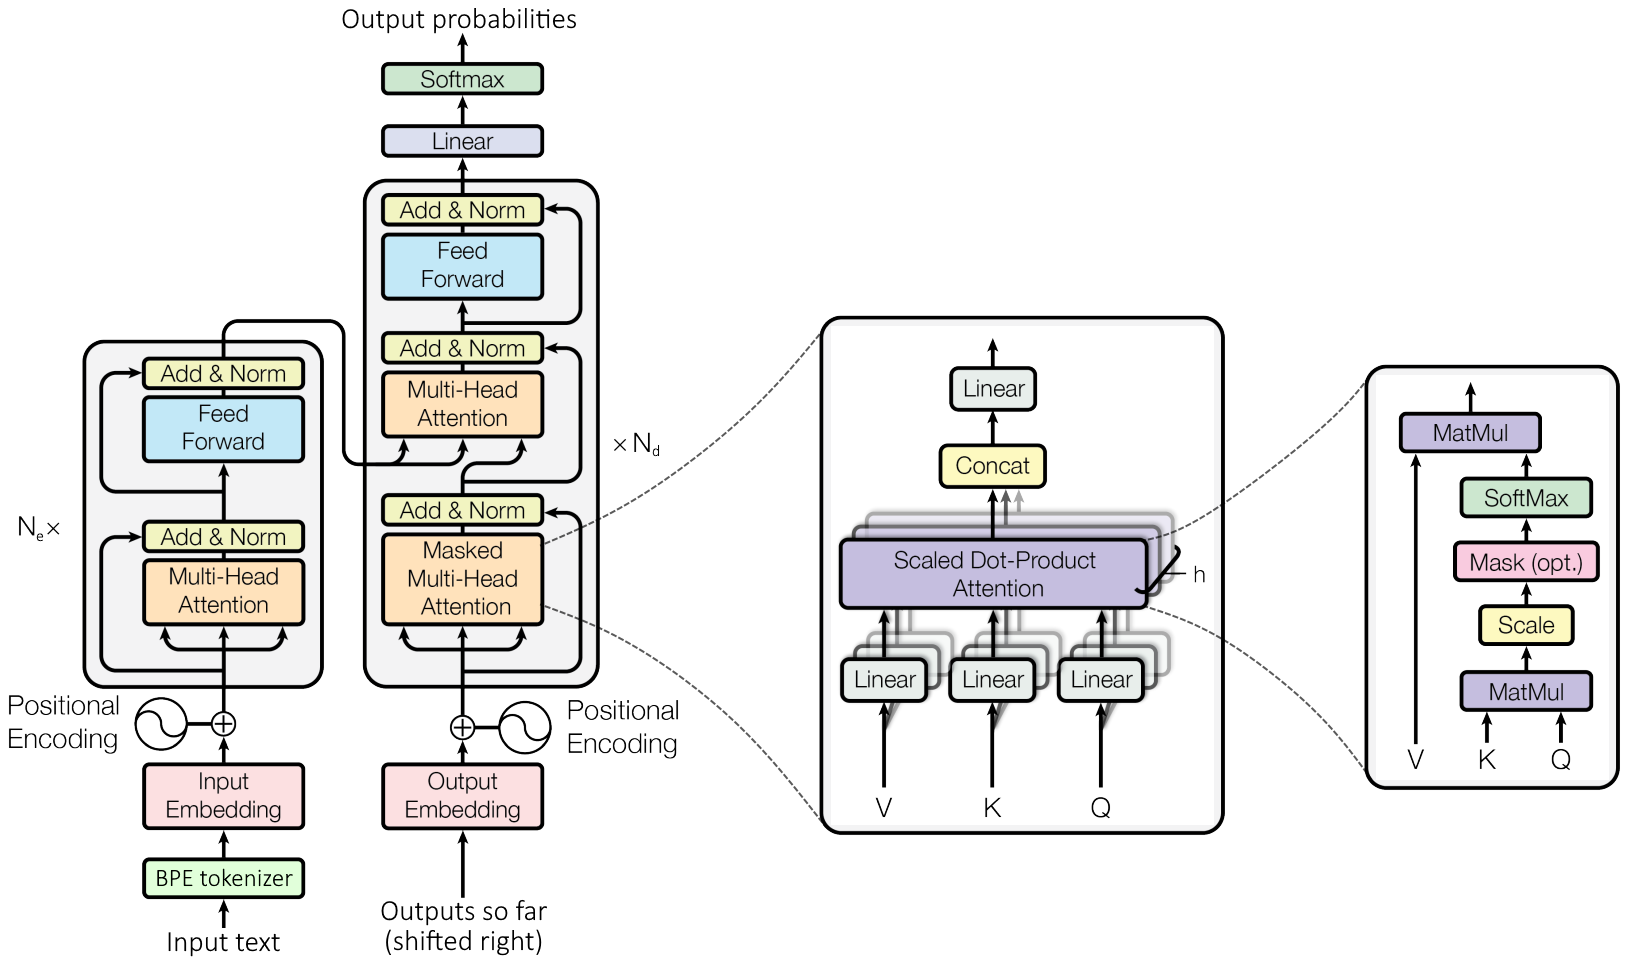
\includegraphics[width=\linewidth]{res/fig/vaswani-transformer}
	\caption[The transformer architecture]{The transformer architecture. Combination of figures by \textcite{vaswani_attention_2017}.}
	\label{fig:transformer}
\end{figure}

\newpage

\subsubsection{Embedded Ti$k$Z code}
\begin{figure}[H]
	\centering
	\begin{tikzpicture}[>=latex] 
		\draw[thin,gray!40] (-6.5,-2.5) grid (6.5,2.5);
		\draw[->] (-2.25,0)--(2.25,0) node[right,yshift=1mm]{good};
		\draw[->] (0,-2)--(0,2) node[above]{emotion};
		\draw[line width=1.5pt,ForestGreen,-stealth](0,0)--(1.5,1.5) node[anchor=south west]{$\vec x$};
		\draw[line width=1.5pt,red,-stealth](0,0)--(-1.5,-1.5) node[anchor=north east]{$-\vec x$};
		\draw[line width=1.5pt,blue,-stealth](0,0)--(-1.5,1.5) node[anchor=north east]{$\vec y$};
	\end{tikzpicture} 
	\caption{Small example of a Cartesian grid in Ti$k$Z.}
	\label{fig:semanticalgebra}
\end{figure}


\subsubsection{Subfigures}
\begin{figure}[h]
	\begin{subfigure}{0.5\linewidth}
		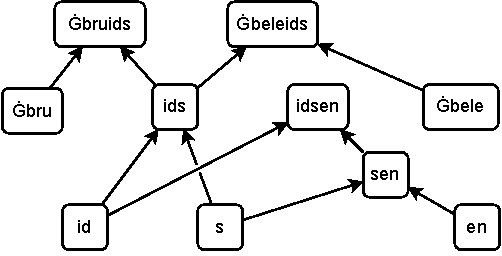
\includegraphics[width=\linewidth]{./res/fig/knockout-before}
		\caption{Before}
	\end{subfigure}
	\hspace{2em}
	\begin{subfigure}{0.5\linewidth}
		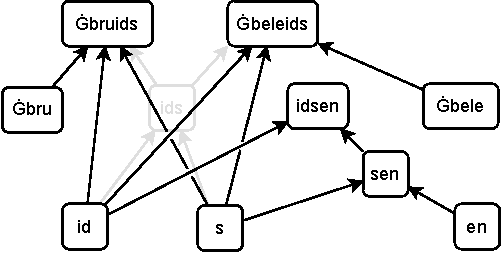
\includegraphics[width=\linewidth]{./res/fig/knockout-after}
		\caption{After}
	\end{subfigure}
	\caption[Visualisation of BPE-knockout]{Visualisation of the changes in part of the BPE merge graph after knockout of the Dutch type \ex{ids}, originating from the merge \ex{id+s}.}
	\label{fig:knockout}
\end{figure}

\begin{landscape}
\mbox{}\vfill 

\subsection{Tables}

\begin{table}[H]
\centering 
\scalebox{0.95}{
\begin{tabular}{c|rr:rr|rr:rr}
                        & \multicolumn{4}{c|}{\thead{morfen}} & \multicolumn{4}{c}{\thead{morfemen}} \\
                        & \thead{gevaren}  & \thead{$\%_\text{tot}$} & \thead{effectief}   & \thead{$\%_\text{gev}$}  & \thead{gevaren}   & \thead{$\%_\text{tot}$} & \thead{effectief}   & \thead{$\%_\text{gev}$}   \\ \hline
\multicolumn{1}{r|}{FP} & $\num{147622}$  &    $61.85\%$    & $\num{16015}$         & $10.85\%$   &  $\num{123743}$    & $51.7\%$     & $\num{11642}$         & $9.41\%$    \\
\multicolumn{1}{r|}{FN} & $\num{16860}$   & $7.06\%$      & $\num{5787}$         & $34.32\%$   & $\num{10077}$    & $4.21\%$     & $\num{2903}$         & $28.81\%$
\end{tabular}
}
\caption[Positive and negative prefix aliasing in e-Lex.]{Positive and negative prefix aliasing in e-Lex. "Hazards" refers to the amount of morphs or morphemes that risk being aliased, and "effective" refers to how many of those materialise while using BPE.}
\label{tab:aliasing}
\end{table}


\begin{table}[h]
\centering 
\scalebox{0.95}{
\begin{tabular}{r|cccccccc}
   & \multicolumn{2}{c|}{\thead{deletie}}        & \multicolumn{2}{c|}{\thead{substitutie}}    & \multicolumn{2}{c|}{\thead{wisseling}}      & \multicolumn{2}{c}{\thead{insertie}}       \\
   & e-Lex & \multicolumn{1}{c|}{NT2Lex} & e-Lex & \multicolumn{1}{c|}{NT2Lex} & e-Lex & \multicolumn{1}{c|}{NT2Lex} & e-Lex & \multicolumn{1}{c}{NT2Lex} \\ \hline 
	Pr & 0.58 & 0.38 & 0.50 & 0.32 & 0.44 & 0.28 & 0.46 & 0.30 \\
	Re & 0.79 & 0.78 & 0.87 & 0.87 & 0.80 & 0.80 & 0.89 & 0.89 
\end{tabular}
}
\caption{Precision en recall van de splitsingspunten die de BPE-tokeniser ingelast in woorden met typo's t.o.v.\ zonder.}
\label{tab:typos}
\end{table}

\begin{table}[h]
\centering
\resizebox{0.8\linewidth}{!}{
\begin{tabular}{lccr|cccccc|cccccc}
& \multirow{3}{*}{\rotatebox{90}{\bfseries Knockout}}& \multirow{3}{*}{\rotatebox{90}{\bfseries Anneal}} &       & \multicolumn{6}{c|}{\thead{morfemen}}                                   & \multicolumn{6}{c}{\thead{lexemen}}                                    \\
&&&       & \multicolumn{3}{c|}{\thead{types}}        & \multicolumn{3}{c|}{\thead{tokens}} & \multicolumn{3}{c|}{\thead{types}}        & \multicolumn{3}{c}{\thead{tokens}} \\
&&& $|V|$ & \thead{Pr} & \thead{Re} & \multicolumn{1}{c|}{\thead{$F_1$}} & \thead{Pr}      & \thead{Re}      & \thead{$F_1$}      & \thead{Pr} & \thead{Re} & \multicolumn{1}{c|}{\thead{$F_1$}} & \thead{Pr}      & \thead{Re}      & \thead{$F_1$}     \\ \hline
BTE & -- & -- & 40.0k & \tgrad{0.52} & \tgrad{0.55} & \multicolumn{1}{c|}{\tgrad{0.54}} & \tgrad{0.55} & \tgrad{0.12} & \multicolumn{1}{c|}{\tgrad{0.19}} & \tgrad{0.38} & \tgrad{0.70} & \multicolumn{1}{c|}{\tgrad{0.50}} & \tgrad{0.36} & \tgrad{0.31} & \tgrad{0.33} \\
BTE-knockout & L & -- & 38.4k & \tgrad{0.56} & \tgrad{0.62} & \multicolumn{1}{c|}{\tgrad{0.59}} & \tgrad{0.68} & \tgrad{0.24} & \multicolumn{1}{c|}{\tgrad{0.35}} & \bfseries \tgrad{0.43} & \tgrad{0.82} & \multicolumn{1}{c|}{\bfseries \tgrad{0.56}} & \bfseries \tgrad{0.56} & \tgrad{0.79} & \bfseries \tgrad{0.66} \\
BTE-knockout-notrivial & L & -- & 39.5k & \tgrad{0.55} & \tgrad{0.61} & \multicolumn{1}{c|}{\tgrad{0.58}} & \tgrad{0.57} & \tgrad{0.15} & \multicolumn{1}{c|}{\tgrad{0.23}} & \tgrad{0.42} & \tgrad{0.80} & \multicolumn{1}{c|}{\tgrad{0.55}} & \tgrad{0.41} & \tgrad{0.42} & \tgrad{0.41} \\
BTE-knockout & M & -- & 35.7k & \bfseries \tgrad{0.61} & \bfseries \tgrad{0.78} & \multicolumn{1}{c|}{\bfseries \tgrad{0.69}} & \bfseries \tgrad{0.82} & \bfseries \tgrad{0.65} & \multicolumn{1}{c|}{\bfseries \tgrad{0.72}} & \tgrad{0.38} & \bfseries \tgrad{0.83} & \multicolumn{1}{c|}{\tgrad{0.52}} & \tgrad{0.26} & \bfseries \tgrad{0.82} & \tgrad{0.39} \\
BTE-knockout-notrivial & M & -- & 37.7k & \tgrad{0.60} & \tgrad{0.73} & \multicolumn{1}{c|}{\tgrad{0.66}} & \tgrad{0.72} & \tgrad{0.38} & \multicolumn{1}{c|}{\tgrad{0.49}} & \tgrad{0.38} & \tgrad{0.80} & \multicolumn{1}{c|}{\tgrad{0.51}} & \tgrad{0.20} & \tgrad{0.42} & \tgrad{0.28} \\
\end{tabular}}
\caption{Evaluatie van BPE-knockout op morfemische en lexemische splitsingspunten in e-Lex.}
\label{tab:knockouttrivial}
\end{table}

\vfill
\end{landscape}

If you want to have tables with numerical results that are within a certain range where one end is good and the other end is bad, you can surround each cell with the \verb|\tgrad{...}| command (short for \emph{table gradient}) to colour the background. One example of such a table is \autoref{tab:knockouttrivial}. Another can be found on page 9 of \textcite{bauwens_bpe-knockout_2024}. If your results originate from a Python program, I highly recommend you use the \href{https://github.com/bauwenst/fiject}{\textsf{fiject}} package to generate your table, including the wrapping of the cells, automatically.
 
\subsection{Algorithms}
Algorithms are floats containing a (non-floating) \verb|algorithmic| environment preceded by a caption and a label. They are numbered automatically, like figures.

To refer to a specific line in a specific algorithm, just put a \verb|\label| at the end of that line and \verb|\autoref| to it. \repo will make sure that the resulting reference links back to the correct line of the correct algorithm.

\autoref{algo:bpe} is a basic algorithm.
\begin{algorithm}[H]
	\caption{Pseudocode BPE}
	\label{algo:bpe}
	\begin{algorithmic}[1]
		\Function{leerBPE}{$\D$, $\tau$}
			%\State Comprimeer $\D$ tot de woordaantallen $W$.
			%\State Splits de woorden in $W$ in karakters, en voeg telkens een EOW-karakter toe.
			\State $\D \gets$ \Call{splitsInWoorden}{$\D$}
			\State $\D \gets$\texttt{[}\Call{splitsInLetters}{$w$} + \texttt{[}\textsc{eow}\texttt{]} $\mid w\in \D$\texttt{]} 
			\State $V \gets \{\ell \in w \mid w \in \D\}$\label{line:bpeinit}
			\State $M \gets \texttt{[]}$
			\While{$|V| < \tau$}
				\State $(x,y) \gets \arg\max\limits_{x,y\in V}$ \Call{aantal}{$\D$, $x$\_$y$}\label{line:bpeargmax}
				\State $\D\gets$ \Call{vervang}{$\D$, $x$\_$y$, $xy$}\label{line:replace}
				\State $V\gets V \cup \{xy\}$
				\State $M\gets M + \texttt{[}(x,y)\texttt{]}$
			\EndWhile
			\vspace{-0.31em}\State\Return $(V,M)$
%			\Stateh\Return $(V,M)$
		\EndFunction
	\end{algorithmic}
\end{algorithm}

You can colour parts of algorithms if you want to highlight them, like in \autoref{algo:bpedropout}.
\begin{algorithm}[H]
	\caption{Pseudocode BPE-dropout}
	\label{algo:bpedropout}
	\begin{algorithmic}[1]
		\Function{gebruikBPEdropout}{$V$, $M$, $w$, $p$}
			\State $w\gets$ \Call{splitsInLetters}{$w$} + \texttt{[}\textsc{eow}\texttt{]}
			\State $i\gets 0$
			\While{$i < |M|$}
				\State $(x,y) \gets M[i]$
				\State $i \gets i + 1$   % i never goes down again.
				\If{$x$\_$y \in w$}
					{\color{blue}
					\If{\Call{random}{0,1} $ < p$}
						\State $w \gets$ \Call{vervang1}{$w$, $x$\_$y$, $xy$}
						\State $i \gets 0$
					\EndIf
					}
				\EndIf
			\EndWhile
			\Statey \Return \texttt{[}\Call{index}{$V$, $t$} $\mid t \in w$\texttt{]}
		\EndFunction
	\end{algorithmic}
\end{algorithm}

\newpage

You can also space out two lines by putting a \verb|\vspace| in between them, like I do to separate two functions in \autoref{algo:kudo}.
\begin{algorithm}[H]
	\caption{Pseudocode ULM}
	\label{algo:kudo}
	\begin{algorithmic}[1]
		\Function{leerULM}{$\D$, $\tau$, $\eta$}
			\State $V \gets $ \Call{alleSubstrings}{$\D$}
			\State $\vec p = (p_1,\hdots,p_{|V|}) \gets (\tfrac{1}{|V|},\hdots,\tfrac{1}{|V|})$
			\While{$|V| > \tau$}
				\State $\vec p \gets$ \Call{herschat}{$\D$, $V$, $\vec p$}
				\State $\Delta\vec{\mathcal L} \gets \vec 0$\Comment{Totale log-likelihoodafname per type}
				\For{$s\in \D$}
					\State $P_s \gets 0$
					\State $\Delta\vec{P}_s \gets \vec 0$  \Comment{Kansafname in $s$ per type}
					\For{$\zeta \in$ \Call{segmentaties}{$s$, $V$}}
						\State $P_\zeta \gets \displaystyle\prod_{t\in \zeta} p_t$\label{line:ulm}  \Comment{Kans van de zinsegmentatie...}
						\State $P_s \gets P_s + P_\zeta$
						\For{$t\in \zeta$}
							\State $\Delta\vec{P}_s[t] \gets \Delta\vec{P}_s[t] + P_\zeta$  \Comment{...valt weg als $t$ wegvalt.}
						\EndFor
					\EndFor 
					\Stateh $\Delta\vec{\mathcal L} \gets \Delta\vec{\mathcal L} + \ln(P_s) - \ln(P_s - \Delta\vec P_s)$  
				\EndFor
				\Statey $V\gets$ \Call{sorteerAflopend}{$V$, $\Delta\vec{\mathcal L}$}  
				\State $V \gets V$\co{[}$0:\eta|V|$\co{]}  \Comment{Weinig likelihood weggevallen $\Rightarrow$ niet nodig}
			\EndWhile
			\Statey \Return $(V,\vec p)$
		\EndFunction
		\vspace{1em}
		\Function{gebruikULM}{$w$, $V$, $\vec p$}
			\State \textsl{Voorwaartse fase (iteratieve i.p.v.\ recursieve viterbi):}
			%\State $m\gets \max\{|t| \mid t\in V\}$
			\State $\ell_1 \hdots \ell_{|w|} \gets -\infty$  \Comment{Beste score tot nu toe gezien door substring $w$\listindex{$1:i$}}
			\State $t_1 \hdots t_{|w|} \gets \unk$  \Comment{Beste eindtoken tot nu toe voor substring $w$\listindex{$1:i$}}
			\For{$i = 1\hdots |w|$}
				%\For{$j = i+1\hdots \min\{i+m, |w|\}$}
				\For{$j = i+1\hdots |w|$}
					\State $t\gets w$\listindex{$i:j$} 
					\If{$t\in V$}
						\State $\ell \gets\ell_i + \ln p_t$
						\If{$\ell > \ell_j$}
							\State $\ell_j \gets \ell$
							\State $t_j \gets t$
						\EndIf 
					\EndIf 
				\EndFor 
			\EndFor 
			\Stateh \textsl{Achterwaartse fase (viterbi-tracé):}
			\State $T\gets$ \co{[]}
			\State $i\gets |w|$
			\While{$i > 0$}
				\State $T \gets$ \co{[}$t_i$\co{]} + $T$
				\State $i \gets i - |t_i|$
			\EndWhile
			\Statey \Return $T$
		\EndFunction
	\end{algorithmic}
\end{algorithm}

\repo defines the two algorithm commands \verb|\Statey| and \verb|\Stateh| which are necessary at some points in an algorithm to connect the indent lines together (e.g.\ after an early return statement). See examples in the source code of \autoref{algo:knockout}.
\begin{algorithm}[H]
	\caption{Knockout: verwijdering van een type uit de BPE-mergegraaf}
	\label{algo:knockout}
	\begin{algorithmic}[1]
		\Function{knockout}{$V$, $M_i$, $M_o$, $\ft$}
			\If{$|M_i(\ft)| = 0$} \Comment{$\ft$ deel van het alfabet}
				\State\Return $(V, M_i, M_o)$
			\EndIf
			\Statey $\{m_\text{old}\} \gets M_i(\ft)$
			\State $o_1,\hdots, o_n \gets$ \Call{ouders}{$m_\text{old}$}
			\For{$i \in 1\hdots n$}
				\State $M_o(o_i) \gets M_o(o_i) \setminus \{m_\text{old}\}$  \Comment{elke ouder vormt $\ft$ niet meer}
			\EndFor \vspace{-0.22em}
			\ForAll{$(q,(t_1, \hdots, \ft, \hdots, t_m)) \in M_o(\ft)$}
				\State $m_\text{new} \gets (q, (t_1,\hdots, o_1, \hdots, o_n, \hdots, t_m))$
				\State $M_i(t_1\hdots \ft \hdots t_m) \gets \{m_\text{new}\}$  \Comment{kind van $\ft$ gevormd door nieuwe merge}
				\For{$i \in 1\hdots n$}
					\State $M_o(o_i) \gets M_o(o_i) \uni\, \{m_\text{new}\}$  \Comment{elke ouder van $\ft$ vormt nu dit kind}
				\EndFor
			\EndFor
			\Statey $V \gets V \setminus \{\ft\}$
			\State $M_i(\ft) \gets \{\}$
			\State $M_o(\ft) \gets \{\}$
			\State \Return $(V, M_i, M_o)$
		\EndFunction
	\end{algorithmic}
\end{algorithm}


\section{Boxes/frames}
Use the \verb|mdframed| environment for creating boxes around your text that are breakable across pages. \repo comes with a couple of styles for these boxes: for example, \verb|style=basic| adds a nice light grey background to your box.

\begin{mdframed}[frametitle={A note about screens}, style=basic,  innertopmargin=0.7em]
	On some screens, you may not see some of the edges of these default boxes. They will, however, appear when you zoom in, when you buy a higher-resolution monitor, and when you print your work on paper.
\end{mdframed}

You can make a box wider than the page margin allows by nesting an \verb|adjustwidth| inside the box. Also, you can wrap a box inside a figure to make it float.
\begin{figure}[h]
	\begin{mdframed}[backgroundcolor=black!5, innertopmargin=-0.6em]
	\begin{adjustwidth}{0cm}{-1cm}
			\begin{equation*}\begin{aligned}
			&\text{invoertekst} \xrightarrow{\text{sanitiser}} \text{tekst} \xrightarrow{\text{pre-tokeniser}} \text{woorden en leestekens} \xrightarrow{\text{tokeniser}} \text{tokens} \xrightarrow{\text{vocab}} \text{id's} \\ &\xrightarrow{\text{LUT}} \text{embeddings} {\color{gray} \,\xrightarrow{\text{model}} \text{kansmassa's} \xrightarrow{\text{decoder}}\, } \text{id's} \xrightarrow{\text{vocab}^{-1}} \text{tokens} \xrightarrow{\text{tokeniser}^{-1}} \text{uitvoertekst}
		\end{aligned}\end{equation*}
	\end{adjustwidth}
	\end{mdframed}
	\caption{NLP pipeline for models with text as output}
	\label{fig:pipeline}
\end{figure}

Here is an example of a breaking box.
\begin{mdframed}[backgroundcolor=black!5]
Some tips about frames:
\begin{enumerate}
	\item You can have frames with no title.
	\item If you want to have a footnote in a frame, use a \verb|\footnotemark| where you want the number to be, and then \emph{outside} of the frame, add \verb|\footnotetext{...}| to declare the text. Kind of like this.\footnotemark 	
	\item If you want to add a figure with a numbered caption, it can't float, so you have to use a \verb|center| environment instead, and to indicate that it's a figure caption, use \verb|\captionof{figure}{...}|.
\end{enumerate}

\begin{center}
	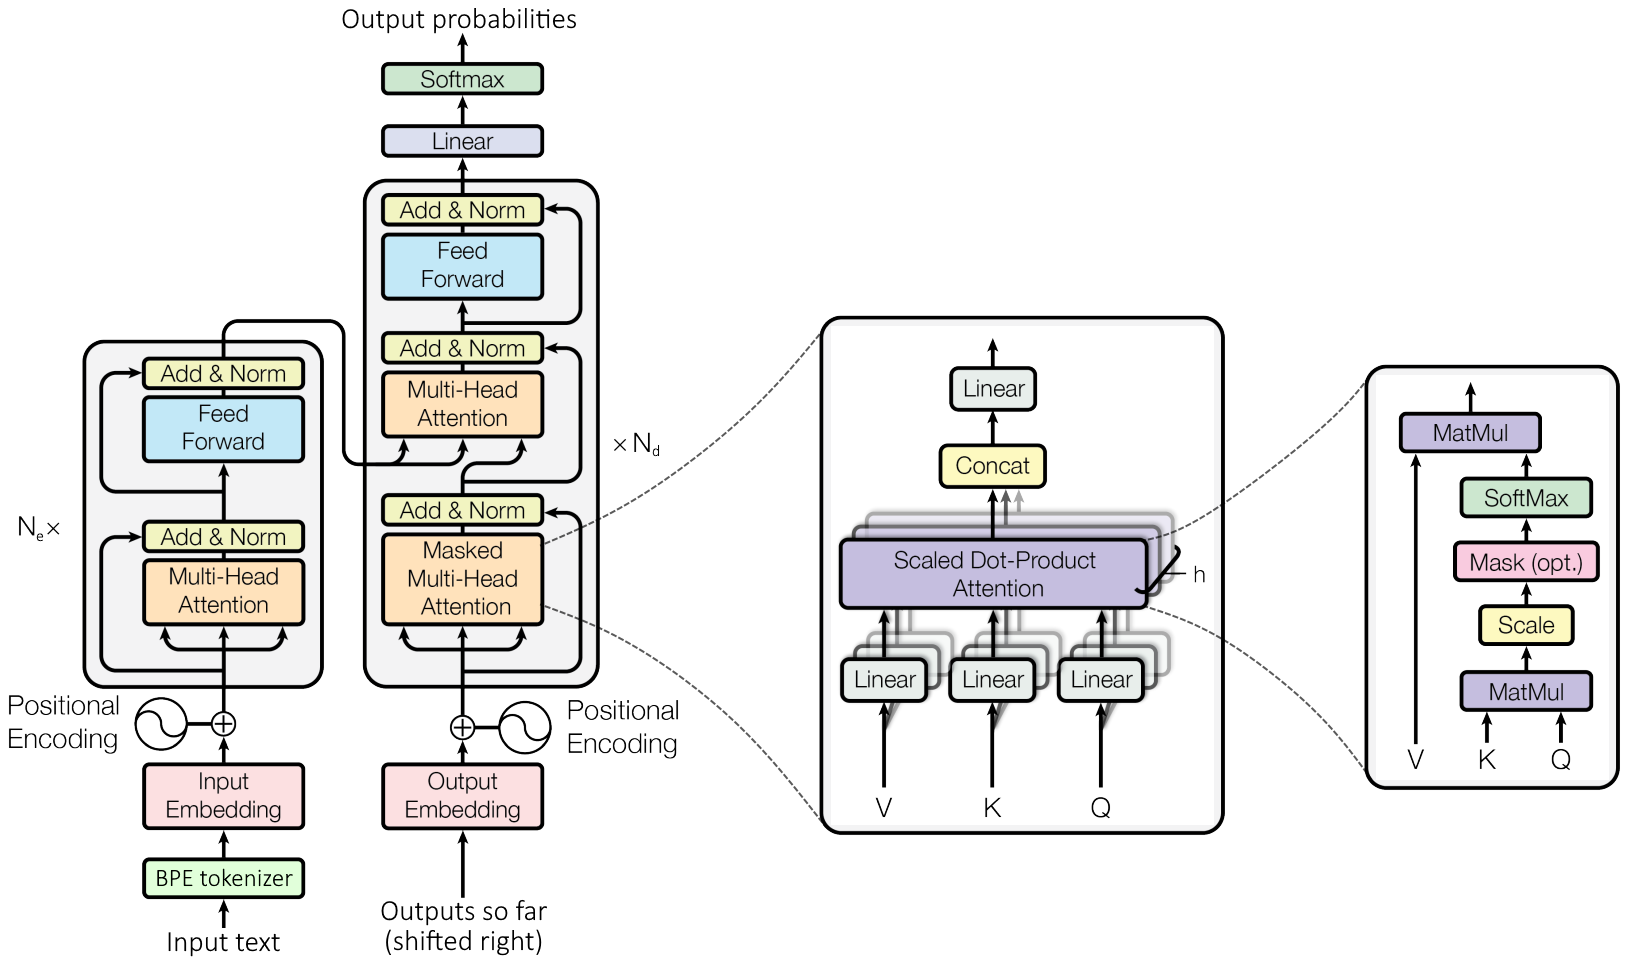
\includegraphics[width=0.75\linewidth]{res/fig/vaswani-transformer}
	\captionof{figure}{Unfloating figure}
\end{center}

\end{mdframed}

\footnotetext{This footnote text belongs to the last footnote mark that was placed.}


\begin{figure}[H]
\begin{mdframed}[backgroundcolor=black!5]
\begin{adjustwidth}{0cm}{-1cm}
\scalebox{0.8}{
\begin{tikzpicture}[
     myboxtext/.style={rectangle, draw, minimum width=1.4em, minimum height=10mm, text depth=0mm, text height=1em},  % "Text height" needed to align labels vertically https://tex.stackexchange.com/a/529480/203081
     myboxarrows/.style={rectangle, draw, minimum width=9.5mm, minimum height=10mm}
 ]
 % Inspired by https://tex.stackexchange.com/a/179753/203081
 \newcommand{\randarrow}{\tikz{
     % random direction and length
     \pgfmathsetmacro\angle{rnd*360}
     \pgfmathsetmacro\halflen{2*(rnd-0.5)*0.15 + 0.3}  % When this value is 0.5, the arrow is 10mm long.
     \draw[line width=1.25pt,-stealth,color=black] (0,0) +(\angle:-\halflen) -- +(\angle:\halflen);}
 }
 
 \def\tokens{
     \textunderscore{}Rob/3663, BER/14334, T/342, 's/167, \textunderscore{}B/138, PE/14388, -/19, to/2751, ken/859, iser/8468, \textunderscore{}split/18486, ste/369, \textunderscore{}dit/52, \textunderscore{}voorbeeld/1403, \textunderscore{}el/4241, o/169, qu/2237, ent/666, ./4
 }
 \edef\tokenAmount{0}  % No, you can't just calculate the length of the above array. I struggled for a whole hour trying to put the result of a function call that did that into a variable that would be allowed by the rectangle below.

 \def\origin{3.1em}

 \node[anchor=west] at (0,\origin) {RobBERT's BPE-tokeniser splitste dit voorbeeld eloquent.};

 \def\origin{0em}

 \node (node0) at (0,\origin) {};
 \foreach \token/\id [count=\x] in \tokens {
     \pgfmathsetmacro{\prevx}{\x-1}
     
     \node[right=-0.15mm of node\prevx, fill=white] (node\x) [myboxtext] {\token};
     \node[below=5mm of node\x.center] {\footnotesize \x};
     \xdef\tokenAmount{\x}
 }
 \draw[ultra thick] (node1.south west) rectangle (node\tokenAmount.north east);

 \def\origin{-5em}

 \node (inode0) at (0,\origin) {};
 \foreach \token/\id [count=\x] in \tokens {
     \pgfmathsetmacro{\prevx}{\x-1}
 
     \node[inner sep=0mm,right=0mm of inode\prevx, fill=white] (inode\x) [myboxarrows]  {\footnotesize\id };
     \node[below=5mm of inode\x.center]  {\footnotesize \x};
 }
 \draw[ultra thick] (inode1.south west) rectangle (inode\tokenAmount.north east);

 \def\origin{-10em}

 \pgfmathsetseed{34678901}
 \node (anode0) at (0,\origin) {};
 \foreach \token/\id [count=\x] in \tokens {
     \pgfmathsetmacro{\prevx}{\x-1}
 
     \node[right=0mm of anode\prevx, fill=white] (anode\x) [myboxarrows]  { };
     \node[below=5mm of anode\x.center]  {\footnotesize \x};
     \node at (anode\x.center) { \randarrow };
 }
 \draw[ultra thick] (anode1.south west) rectangle (anode\tokenAmount.north east);
\end{tikzpicture}
}
\end{adjustwidth}
\end{mdframed}
\caption[Data formats at the interfaces inside an NLP system]{Data formats at the interfaces inside an NLP system. Top to bottom: what the tokeniser sees (characters), what the vocabulary sees (subwords), what the embedding matrix sees (token-IDs), and what a neural model sees (embedding vectors).}
\label{fig:interfaces}
\end{figure}


\section{Code}
When you typeset code, it is a crime to use the \co{listings} package.

The \TeX{}studio settings that come with \repo allow typesetting with the \verb|minted| package out of the box. You can do this inline with the \verb|\mintinline| command, like \mintinline{python}|bytes(corpus, "utf-8")|, you can load code from a file with \verb|\inputminted| like
\inputminted[linenos]{python}{./res/code/hello.py}

and finally, if it's a very small example snippet, you can also just embed your code in the \verb|minted| environment in your \LaTeX{} document:
\begin{minted}[linenos]{python}
def example() -> int:
    return 1
\end{minted}

\section{Menus}
If, for some reason, you need to tell readers how to navigate through a digital menu, you can do so with \verb|\menu[,]{a,b,c,d,e}|. For example, my thesis contained the menu path
\menu[,]{Create Lexicon, Dutch Lemmas, StrucLab, Ok, Ok, Include Word, Ok}

\section{Controlling line breaks}
These commands are not specific to \repo, but I'll mention them anyway. \textbf{Note:} you probably shouldn't use these unless you are finished writing your thesis.
\begin{itemize}
\item If you want to force text to the next line and leave the rest of the line blank without triggering a blank line, insert \verb|\\|.
\item If you want a word to be more likely to be hyphenated at a certain point, add \verb|\-| at that point in the word. This helps in Dutch compounds, which \LaTeX{} sometimes can't hyphenate, e.g.\ \verb|rivier\-beddings\-door\-sneden|.
\item If you want to protect a word against being hyphenated at the edge of a line, surround it by \verb|\mbox{}|.
\item If you want a certain space to never be the end a line, replace it by \verb|~|.
\item If you want a certain space to be more likely to be the end of a line, replace it by \verb|\allowbreak{}|.
\item If you want a word to be able to exceed the edge of the line, use \verb|\rlap|.
\end{itemize}


\section{Todos}
Because the \co{todonotes} \LaTeX{} package is evil, \repo defines its own rudimentary \verb|\todo{...}| command that will show up as red boxes in the margin of your thesis.\todo{Like this.}

	% !TeX spellcheck = nl_NL
\chapter{Summary \& Conclusion}
There is a difference between the summary and the conclusion.
\begin{itemize}
	\item The summary recapitulates what the thesis covered. For each chapter, you say what its purpose was, but \emph{also} give concrete take-aways the reader should remember from the different parts.
	\item The conclusion answers the research questions briefly, and then looks into the future of the field of study.
\end{itemize}

\section{Summary}
\autoref{chap:intro} explained how \repo is like a short thesis that can be read as source code or as a PDF. It also explained what a thesis introduction should accomplish.
\segsep
\autoref{chap:literature} gave a brief overview of alternative thesis templates. We saw that the most important existing template was kulemt and the reasons why I don't like it.
\segsep
\autoref{chap:questions} converged on the fundamental question, which is whether we can make an engineering master's thesis template better than kulemt.
\segsep 
\autoref{chap:bauwemt} walked through the installation of \repo. It then discussed how the project is organised into a preamble, a main text, and resources. Finally, it also gave practical advice on how to write the thesis, in particular stressing that you should always save except while compiling.
\segsep
\autoref{chap:functionality} lastly showed off all the different outputs that can be achieved out of the box with \repo. Apart from going over existing commands for equation alignment, hyperlinking, citations, figures, tables, algorithms, boxes, code, menu navigation, and line break control, we also covered new commands like \verb|blockquote| for nicer quotation, \verb|\pagelabel| for correctly linking back to the page of an object, and \verb|\emph*| and \verb|\Emph*| for adding terms to the index.

\section{Conclusion}
I asked in \autoref{chap:questions} if a better template could be crafted than kulemt. From all of the above, the answer is yes.

\section{Future work}
You can now provide the reader with a list of research questions you yourself would like to see answered, knowing all that you know now and having improved the state-of-the-art. Of course, \repo is perfect and hence there is no future work \co{;-)}.

	
	\appendix  			% Needed so that appendix is detectable by apptools in Theme.tex.
	\begin{appendices}  % Needed to add the "Appendix" prefix in the ToC.
	\part{\textsc{\mdseries{Appendices}}}\label{pt:apx}
%	\input{text/apx/Viterbi.tex}
%	\input{text/apx/Datasets.tex}
%	\input{text/apx/Attachments.tex}
	\end{appendices}
	
	\backmatter
	% Since \backmatter doesn't reset the page number or change page style, I thought it might be cool to continue mainmatter numbering but in Roman style https://tex.stackexchange.com/q/56131/203081
	%\renewcommand{\thepage}{\alph{page}}
	% Actually, nah, I want to use \alph and start from a. https://tex.stackexchange.com/a/56133/203081
	\pagenumbering{alph}
	\chapter{\sourcesname}
% "heading=bibintoc" creates a chapter, "heading=subbibintoc" creates a section. Both cause \printbibliography to appear in the table of contents.
\printbibliography[heading=subbibintoc, title={\refname}, category=cited]
\printbibliography[heading=subbibintoc, title={\furtherrefname}, notcategory=cited]

\hyphenchar\font=-1  % Stop hyphenation https://tex.stackexchange.com/a/5039/203081
\printindex
\end{document}